\documentclass[11pt]{article}

\usepackage[margin=1in]{geometry}
\usepackage{amsmath,amssymb,mathtools}
\usepackage{booktabs}
\usepackage{enumitem}
\usepackage{array}
\usepackage{graphicx}
\usepackage{caption}
\usepackage{xcolor}
\usepackage[hidelinks]{hyperref}

\graphicspath{{figures/}}
\captionsetup{font=small,labelfont=bf}

\definecolor{kicol}{RGB}{31,143,107}
\definecolor{boxbg}{RGB}{238,246,242}
\definecolor{rmkbg}{RGB}{244,244,244}

\newcommand{\plain}[1]{\par\smallskip\noindent{\color{kicol}\textbf{In plain words.}}\ \textit{#1}\par\smallskip}
\newcommand{\problembox}[1]{%
  \par\smallskip\noindent\fcolorbox{kicol}{boxbg}{%
  \parbox{0.965\linewidth}{\smallskip\textbf{\color{kicol}What problem is solved here.}\ \ #1\smallskip}}\par\smallskip}
\newcommand{\remark}[2]{%
  \par\smallskip\noindent\colorbox{rmkbg}{%
  \parbox{0.965\linewidth}{\smallskip\footnotesize\textbf{#1}\ \ #2\smallskip}}\par\smallskip}
\newcommand{\bridge}[1]{\par\noindent\textit{#1}\par\medskip}

\newcommand{\D}{\mathrm{D}}
\newcommand{\imag}{\mathrm{i}}
\newcommand{\Real}{\operatorname{Re}}
\newcommand{\Imag}{\operatorname{Im}}
\newcommand{\Mae}{M_e}
\newcommand{\Ree}{\mathit{Re}}
\renewcommand{\bar}[1]{\overline{#1}}
\newcommand{\hatu}{\hat{u}}
\newcommand{\hatv}{\hat{v}}
\newcommand{\hatT}{\hat{T}}
\newcommand{\hatp}{\hat{p}}
\newcommand{\hatq}{\hat{q}}
\newcommand{\nuR}{\nu_{\!R}}

\title{\textbf{Linear Stability Theory, From Scratch}\\[3pt]
\large A complete, self-contained guide to formulating and numerically solving the\\
compressible boundary-layer stability problem --- as implemented in \texttt{pyMack}}
\author{Personal reference note}
\date{\today}

\begin{document}
\maketitle

\begin{abstract}
\noindent This note explains --- assuming \emph{no prior exposure} to stability theory or spectral
methods --- everything needed to understand and re-implement a compressible Linear Stability Theory
(LST) solver. Every symbol is defined, every matrix is opened up (including the full block structure and
which terms carry the eigenvalue), the node ordering and boundary-condition row indices are stated
explicitly, and a fully worked numerical example with real solver output is given. All equations,
coefficients, and parameter defaults are transcribed from the actual code in \texttt{pymack/}, cited by
file throughout, so the document doubles as a code$\leftrightarrow$math map.
\end{abstract}

\tableofcontents
\bigskip

\noindent\textbf{How to read this.} Sections build strictly on one another. Boxes marked
{\color{kicol}\textbf{``What problem is solved here''}} state, at each stage, exactly which equation,
which boundary conditions, and which unknown (the eigenvalue) are involved. \emph{In plain words} notes
give the intuition; grey \textsf{Remark} asides hold secondary or fallback detail you can skip on a first
read.

\paragraph{Notation.} Overbars are mean (base-flow) quantities; hats are complex disturbance amplitudes.
The continuous wall-normal amplitude is $\hatq(y)=(\hatu,\hatv,\hatT,\hatp)$; its discrete (stacked,
grid-sampled) form is the vector $\boldsymbol\phi$. A prime on a mean quantity is $\D\equiv\mathrm d/\mathrm dy$.
\begin{center}\footnotesize
\renewcommand{\arraystretch}{1.18}
\begin{tabular}{@{}ll@{\hspace{1.4em}}ll@{}}
\toprule
\multicolumn{2}{@{}l}{\textbf{Base flow \& transport}} & \multicolumn{2}{l}{\textbf{Disturbance / eigenvalue}}\\
$\bar U,\bar T,\bar\rho{=}1/\bar T$ & mean velocity, temp., density & $\hatq;\ \boldsymbol\phi$ & amplitude (cont.; discrete), Eq.~\eqref{eq:ansatz}\\
$\bar\mu,\bar\kappa$ & viscosity, conductivity & $\hatu,\hatv,\hatT,\hatp$ & velocity/temp./pressure amplitudes\\
$C{=}\bar\mu/\bar T,\ K,\ B$ & transport groups, \S\ref{sec:base} & $\alpha,\ \omega$ & wavenumber, frequency\\
\multicolumn{2}{@{}l}{\textbf{Scales \& parameters}} & $c{=}\omega/\alpha$ & complex phase speed; $c_r,c_i$ its parts\\
$\Mae,\ \Ree,\ \mathit{Pr},\ \gamma$ & Mach, Reynolds, Prandtl, $c_p/c_v$ & $\omega_i{=}\alpha c_i$ & temporal growth rate, Eq.~\eqref{eq:tgrowth}\\
$L^*{=}\sqrt{\nu_e x/U_e}$ & Mack length, Eq.~\eqref{eq:Lstar} & $\sigma{=}-\Imag(\alpha)$ & spatial growth rate, Eq.~\eqref{eq:sgrowth}\\
$R{=}\sqrt{Re_x},\ F$ & Mack Reynolds, reduced freq., Eq.~\eqref{eq:RF} & $M_{\rm rel}$ & relative Mach number, \S\ref{sec:mechanisms}\\
$\alpha_L{=}\alpha L^*,\ \delta^*,\theta$ & scaled wavenumber, thicknesses & $N,\ n{=}N{+}1$ & collocation points; grid size\\
\bottomrule
\end{tabular}
\end{center}
\noindent{\footnotesize\textbf{Operator shorthands:}\ $D_1,D_2$ derivative matrices (Eq.~\ref{eq:Dmats});\
$\nuR{=}1/(\Ree\bar\rho)$;\ $\mathcal C_\kappa,\mathcal C_d,d_R$ conduction/dissipation prefactors;\
$\mathcal L_c$ conduction operator;\ $A,B$ (temporal) and $C_0,C_1,C_2$ (spatial) operator blocks.\par}

%=====================================================================
\part*{Part I --- The idea}
\addcontentsline{toc}{section}{Part I --- The idea}
%=====================================================================

\section{What stability theory asks, and the plan}\label{sec:idea}
A laminar boundary layer is a smooth, steady flow that eventually becomes turbulent. The first stage of
that process is the amplification of tiny disturbances --- noise, roughness, free-stream turbulence ---
always present in a real flow. \emph{Linear} Stability Theory asks the cleanest version of the question:

\begin{quote}
If we add one infinitesimally small wave to the laminar flow, does that wave \textbf{grow} or
\textbf{decay} as it travels?
\end{quote}

We will write that small wave as $q'(x,y,t)$ --- shorthand for the collection of all disturbance
quantities (velocity, temperature, pressure; defined precisely in Eq.~\eqref{eq:split}). ``Infinitesimal''
is the key word: if $q'$ is small enough, products of small quantities are negligible and its governing
equations become \emph{linear}.

\paragraph{Why this becomes an eigenvalue problem.} After linearising, the coefficients of the equations
depend only on the wall-normal coordinate $y$ (Part III). Because they are \emph{constant in $x$ and $t$},
substituting a single trial wave $q'\propto e^{\imag(\alpha x-\omega t)}$ turns every $x$- and
$t$-derivative into multiplication by a constant; the equations then no longer involve $x$ or $t$ at all,
only the wave's wall-normal shape. The requirement that a \emph{non-zero} shape exist is precisely an
\textbf{eigenvalue condition}, made concrete in \S\ref{sec:temporal}.

\plain{An eigenvalue problem is the statement ``$\mathsf{A}\hatq=\lambda\hatq$'': for most $\lambda$ the
only solution is $\hatq=0$ (no wave), but for special values $\lambda$ --- the eigenvalues --- a non-zero
shape $\hatq$ (the eigenfunction) exists. Here the eigenvalue carries the growth rate, so its sign tells us
grow or decay.}

\begin{figure}[h]\centering
  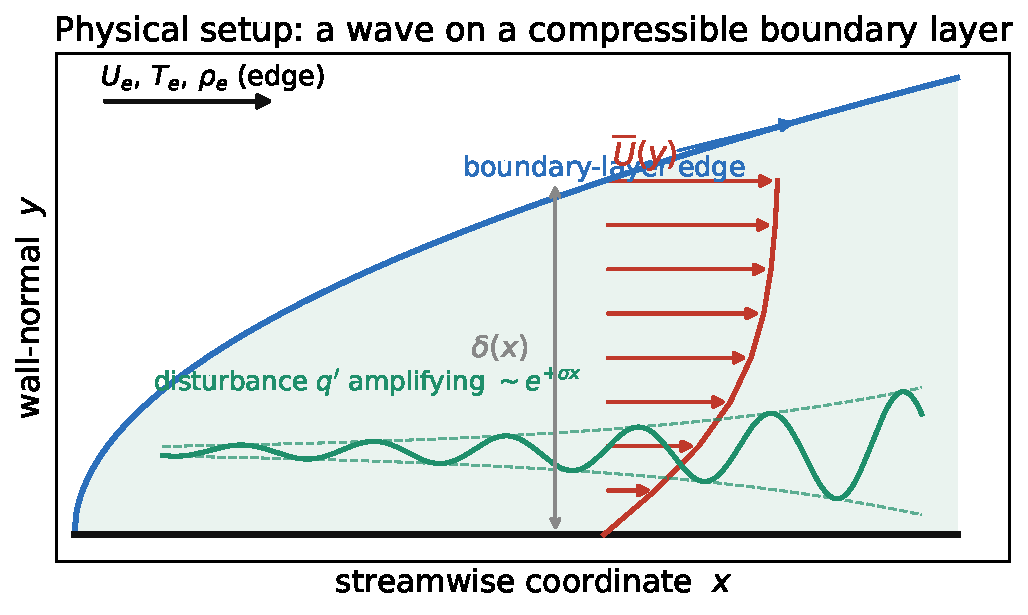
\includegraphics[width=0.86\linewidth]{fig_setup.pdf}
  \caption{The physical setup. A steady compressible boundary layer grows along a wall; its mean velocity
  $\bar U(y)$ and temperature $\bar T(y)$ vary across the layer of thickness $\delta(x)$. LST tracks one
  small disturbance $q'(x,y,t)$ riding in this layer and asks whether it amplifies downstream.}
\end{figure}

LST is one stage of a longer story (Figure~\ref{fig:roadmap}): disturbances first \emph{enter} the layer
(receptivity), then grow linearly (LST --- this document), then break down nonlinearly to turbulence. We
treat only the linear-growth stage; \S\ref{sec:scope} states exactly what that leaves out.

\begin{figure}[h]\centering
  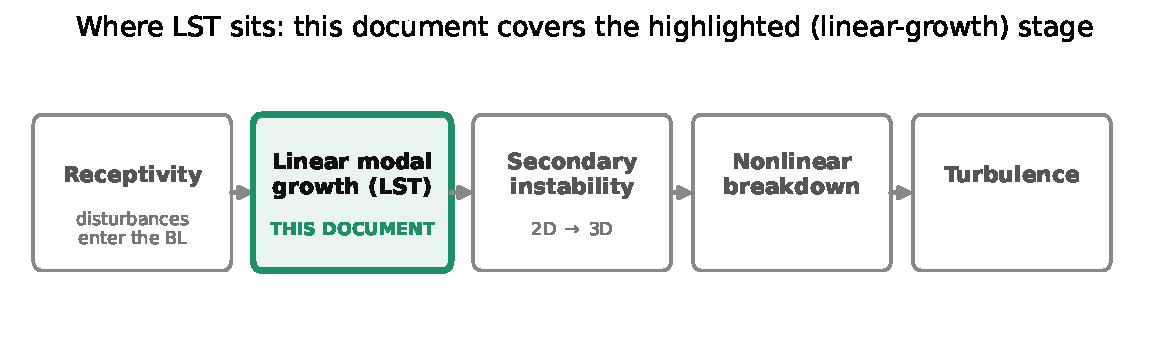
\includegraphics[width=0.95\linewidth]{fig_transition_roadmap.pdf}
  \caption{The transition process. This document covers the highlighted linear-modal-growth stage (which
  produces the $e^N$ amplification); receptivity and nonlinear breakdown are separate problems
  (\S\ref{sec:scope}).}\label{fig:roadmap}
\end{figure}

The computation itself is a short pipeline (Figure~\ref{fig:workflow}):
\begin{enumerate}[nosep,leftmargin=2.2em]
  \item compute the steady \textbf{mean (base) flow} (Part II);
  \item \textbf{linearise} and insert a wave \textbf{ansatz} to get ordinary differential equations in $y$ (Part III);
  \item \textbf{discretise} those ODEs into matrices with Chebyshev collocation (Part IV);
  \item solve the resulting \textbf{eigenvalue problem} for the growth rate (Part V);
  \item sweep parameters to draw \textbf{neutral curves} and integrate \textbf{$N$-factors} (Part VI).
\end{enumerate}

\begin{figure}[h]\centering
  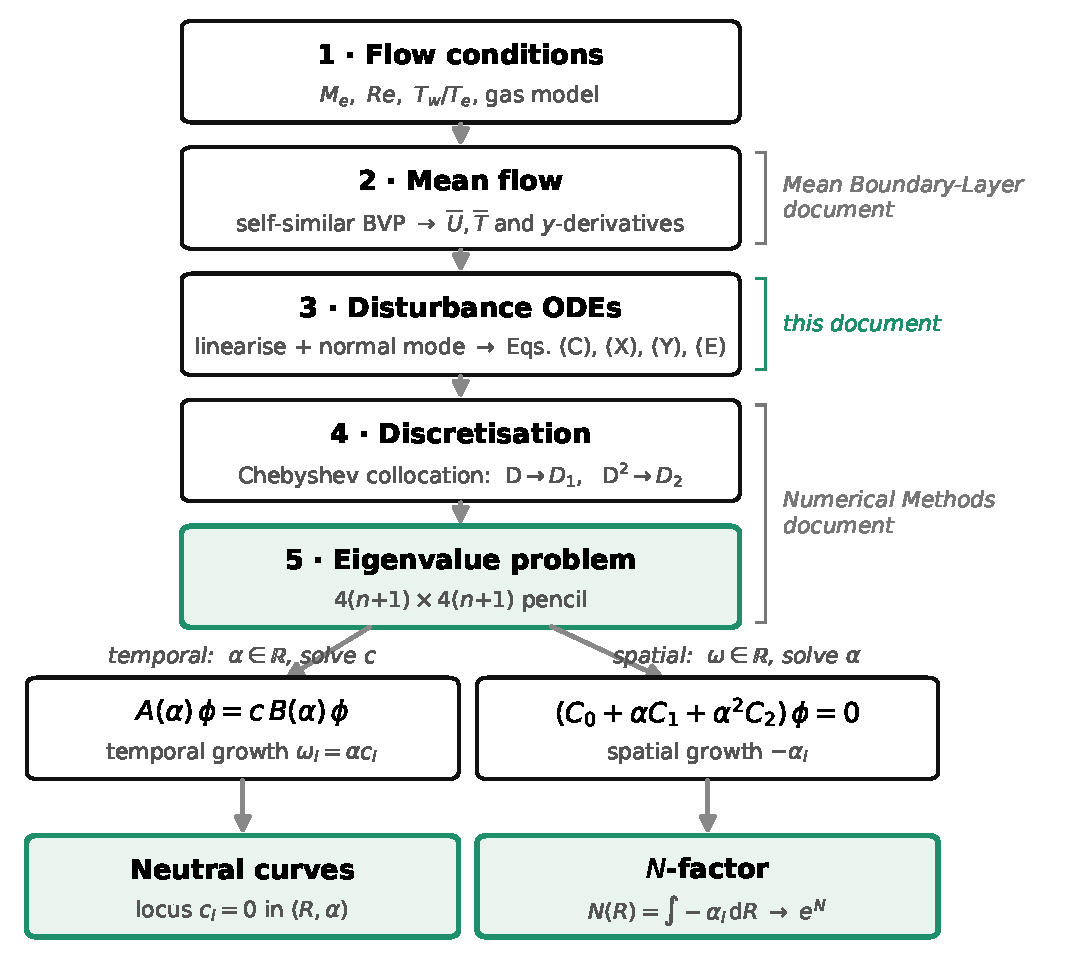
\includegraphics[width=0.6\linewidth]{fig_workflow.pdf}
  \caption{End-to-end workflow. The single eigenvalue solve (stage~5) forks into a \emph{temporal} route
  (real wavenumber $\alpha$ in, complex phase speed $c$ out; used for neutral curves) and a \emph{spatial}
  route (real frequency $\omega$ in, complex $\alpha$ out; used for $N$-factors).}\label{fig:workflow}
\end{figure}

%=====================================================================
\part*{Part II --- The mean flow}
\addcontentsline{toc}{section}{Part II --- The mean flow}
%=====================================================================
\bridge{The disturbance rides on a steady laminar flow, so we need that flow --- and its $y$-derivatives ---
before anything else. This Part computes it.}

\section{Governing equations and non-dimensionalisation}\label{sec:gov}
The flow obeys the compressible Navier--Stokes equations --- conservation of mass, momentum, and energy for
a viscous, heat-conducting perfect gas:
\begin{align}
  \frac{\D\rho}{\D t}+\rho\,\nabla\!\cdot\!\mathbf u &= 0, &&\text{(mass)}\label{eq:ns-mass}\\
  \rho\frac{\D\mathbf u}{\D t} &= -\nabla p+\nabla\!\cdot\!\boldsymbol\tau, &&\text{(momentum)}\label{eq:ns-mom}\\
  \rho\,c_p\frac{\D T}{\D t} &= \frac{\D p}{\D t}+\nabla\!\cdot(\kappa\nabla T)+\Phi, &&\text{(energy)}\label{eq:ns-energy}\\
  p &= \rho R T, &&\text{(state)}\label{eq:ns-state}
\end{align}
where $\mathbf u=(u,v)$ is velocity, $\rho$ density, $T$ temperature, $p$ pressure, $\mu$ viscosity,
$\kappa$ conductivity, $c_p$ specific heat, $R$ the gas constant, and $\D/\D t=\partial_t+\mathbf u\!\cdot\!\nabla$
the material derivative. The two remaining symbols are the Newtonian \textbf{viscous stress tensor} and the
\textbf{dissipation function},
\begin{equation}\label{eq:tauphi}
  \boldsymbol\tau=\mu\Big(\nabla\mathbf u+\nabla\mathbf u^{\mathsf T}-\tfrac23(\nabla\!\cdot\!\mathbf u)\,\mathbf I\Big),
  \qquad \Phi=\boldsymbol\tau\!:\!\nabla\mathbf u .
\end{equation}
We will not need their closed form again: all that matters downstream is that they are linear in velocity
gradients. These four equations are applied \emph{twice} --- once to obtain the steady mean flow (this
Part), once linearised for the disturbance (Part III).

\paragraph{Non-dimensionalisation and default gas constants.} Velocities are scaled by the edge speed
$U_e$, temperature by $T_e$, density by $\rho_e$, viscosity by $\mu_e$, pressure by $\rho_e U_e^2$. Because
the gas is perfect and pressure is nearly uniform across the layer, $\bar\rho=1/\bar T$ in these units.
Three dimensionless groups control everything,
\begin{equation}
  \Mae=\frac{U_e}{\sqrt{\gamma R T_e}},\qquad
  \Ree=\frac{\rho_e U_e L_{\mathrm{ref}}}{\mu_e},\qquad
  \mathit{Pr}=\frac{\mu_e c_p}{\kappa_e},
\end{equation}
with default air values $\gamma=1.4$, $\mathit{Pr}=0.72$, Sutherland constant $S=110.4~\mathrm K$, and
power-law exponent $\omega_\mu\approx0.7$ when the power-law viscosity is used.

\paragraph{The Mack length and Reynolds scales.}\label{sec:Lstar} Boundary layers grow like $\sqrt x$, so
the natural local scale at station $x$ is
\begin{equation}\label{eq:Lstar}
  L^*=\sqrt{\frac{\nu_e\,x}{U_e}},\qquad \nu_e=\frac{\mu_e}{\rho_e}.
\end{equation}
With $L_{\mathrm{ref}}=L^*$ the Reynolds number becomes the square root of the usual one, and a fixed
physical frequency $f$ maps to a reduced frequency $F$ (both \emph{first used in Part VI}, where neutral
curves and $N$-factors consume them):
\begin{equation}\label{eq:RF}
  R=\frac{U_eL^*}{\nu_e}=\sqrt{Re_x},\quad Re_x=\frac{U_ex}{\nu_e};\qquad
  F=\frac{2\pi f\,\nu_e}{U_e^2};\qquad \omega=F\,R,\quad \alpha_L=\alpha L^* .
\end{equation}
$R$ is the horizontal axis of every neutral curve and $\alpha_L$ the vertical axis. Conversions live in
\texttt{pymack/scales.py}; the solver itself is dimensionless. A profile may be stored on a $y/\delta^*$ or
a $y/L^*$ grid; the constant $\delta^*/L^*$ converts between them, with $\D\!\mapsto\!(\delta^*/L^*)^{-1}\D$.

\section{The base flow}\label{sec:base}
\problembox{Solve a \emph{boundary-value problem} (BVP) --- not an eigenvalue problem --- for the steady
laminar profiles $\bar U(y),\bar T(y),\bar\rho(y),\bar\mu(y)$ and their $y$-derivatives. A BVP fixes the
data at both ends ($y=0$ and $y\to\infty$) and has a single solution; an eigenvalue problem instead leaves
a parameter free and asks for the special values that admit a non-zero solution. These profiles become the
known coefficients of the disturbance equations.}

For a flat plate the mean flow is \emph{self-similar}: profiles at different $x$ collapse onto one curve in
a stretched coordinate $\eta$. With the dimensionless stream function $f(\eta)$, $f'=\bar U=u/U_e$ (a prime
is $\mathrm d/\mathrm d\eta$), momentum and energy reduce to two coupled ODEs,
\begin{align}
  \big(C\,f''\big)' + f\,f'' &= 0, \label{eq:bl-mom}\\
  \big(B\,\bar T{}'\big)' + f\,\bar T{}' + (\gamma-1)\,\Mae^2\,C\,\big(f''\big)^2 &= 0, \label{eq:bl-energy}
\end{align}
with transport groups
\begin{equation}
  C=\frac{\mu/\mu_e}{T/T_e}\ \text{(Chapman--Rubesin)},\qquad K=\frac{\kappa}{c_p\mu_e},\qquad
  B=\frac{K}{\bar T}\Big(=\tfrac{C}{\mathit{Pr}}\ \text{at constant }\mathit{Pr}\Big).
\end{equation}
The last term in \eqref{eq:bl-energy} is aerodynamic heating --- it makes a hypersonic layer hot near the
wall and couples energy to velocity. The conductivity model is $\kappa=\mu c_p/\mathit{Pr}$ (so
$\bar\kappa=\bar\mu/\mathit{Pr}$ at constant $\mathit{Pr}$); the transport derivatives
$\mathrm d\mu/\mathrm dT$ etc.\ are taken analytically from the chosen viscosity law.

\paragraph{Wall and edge conditions.}
\begin{equation}\label{eq:blbc}
  \underbrace{f(0)=0,\ f'(0)=0}_{\text{no slip}},\quad
  \underbrace{f'(\infty)=1,\ \bar T(\infty)=1}_{\text{match the edge}},\qquad
  \begin{cases}\bar T{}'(0)=0 &\text{(adiabatic wall)}\\ \bar T(0)=T_w/T_e &\text{(isothermal wall)}\end{cases}
\end{equation}
For an adiabatic wall the recovered temperature is the standard result (stated, not derived)
$T_{aw}/T_e=1+\tfrac12(\gamma-1)\sqrt{\mathit{Pr}}\,\Mae^2$. (For a cone, the edge state itself comes first,
from the Taylor--Maccoll equation behind the conical shock; \texttt{taylor\_maccoll\_edge\_state.py}.)

\paragraph{Solution and the coordinate transform.} Equations \eqref{eq:bl-mom}--\eqref{eq:bl-energy} are
solved as a 5-state first-order system $[\,f,\bar U,\bar U',\bar T,\bar T'\,]$ by
\texttt{scipy.integrate.solve\_bvp} (collocation + Newton; \texttt{pymack/baseflow.py}), integrated to
$\eta_{\max}\!\approx\!40$ (well beyond the edge). The similarity coordinate maps to the physical one by
\begin{equation}\label{eq:ytransform}
  \frac{y}{L^*}=\sqrt2\!\int_0^\eta\frac{\bar T}{T_e}\,\mathrm d\eta',\quad
  \frac{\delta^*}{L^*}=\sqrt2\!\int_0^\infty(\bar T-\bar U)\,\mathrm d\eta,\quad
  \frac{\theta}{L^*}=\sqrt2\!\int_0^\infty\bar U(1-\bar U)\,\mathrm d\eta,
\end{equation}
where the displacement thickness $\delta^*$ measures how far the wall effectively pushes the outer flow
outward and the momentum thickness $\theta$ the momentum deficit. The solver returns, on any grid,
$\bar U,\bar U',\bar U'',\ \bar T,\bar T',\bar T'',\ \bar\rho,\ \bar\mu,\ \mathrm d\mu/\mathrm dT,\
\mathrm d^2\mu/\mathrm dT^2,\ \bar\kappa,\ \mathrm d\kappa/\mathrm dT,\ \mathrm d^2\kappa/\mathrm dT^2$.

\remark{Two base-flow implementations.}{\texttt{baseflow.py} contains two equivalent self-similar
formulations sharing the 5-ODE structure above. Equations \eqref{eq:bl-mom}--\eqref{eq:bl-energy} and the
$\sqrt2$ transform \eqref{eq:ytransform} are the \texttt{CompressibleBlasiusProfile} form. The temporal
solver and the worked example of \S\ref{sec:worked} use \texttt{make\_flatplate\_profile}
(\texttt{FlatPlateProfile}; Ozgen \& Kircali transport laws), an alternative normalisation ($f'=\bar U/\bar T$, $\tfrac12$ factors,
$y/L^*=\eta$, no $\sqrt2$). The two give the same physical profiles; only the similarity bookkeeping
differs.}

\begin{figure}[h]\centering
  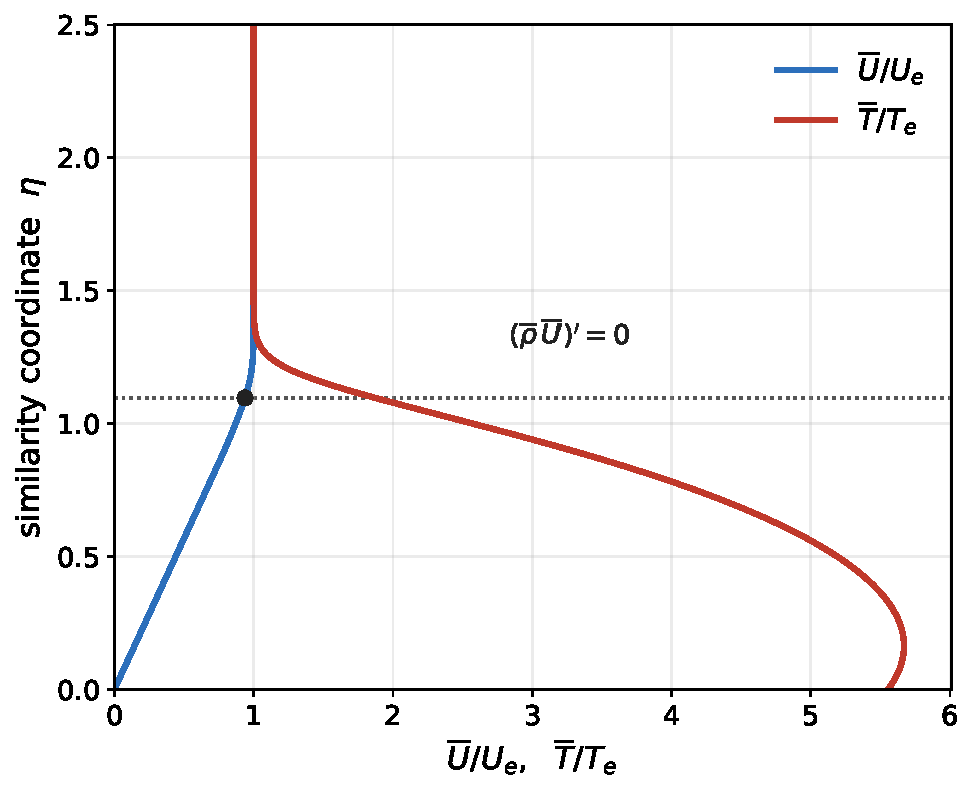
\includegraphics[width=0.55\linewidth]{fig_baseflow.pdf}
  \caption{A computed compressible base flow ($\Mae=4.5$, adiabatic). $\bar U(y)/U_e$ rises monotonically to
  the edge; $\bar T(y)$ bulges near the wall from viscous heating. These curves and their $y$-derivatives are
  the known coefficients $\bar U,\bar T,\dots$ in the disturbance equations. The dotted line marks the
  generalised inflection point (\S\ref{sec:mechanisms}), the seat of the inviscid instability.}\label{fig:baseflow}
\end{figure}

%=====================================================================
\part*{Part III --- The disturbance equations}
\addcontentsline{toc}{section}{Part III --- The disturbance equations}
%=====================================================================
\bridge{We now perturb the mean flow by an infinitesimal wave and reduce the governing PDEs to ordinary
differential equations in $y$ --- the equations the rest of the document discretises and solves.}

\section{Linearisation and the normal-mode ansatz}\label{sec:lin}

\paragraph{Step 1 --- split into mean plus disturbance.}
\begin{equation}\label{eq:split}
  u=\bar U(y)+u',\ v=v',\ T=\bar T(y)+T',\ p=\bar p+p',\ \rho=\bar\rho(y)+\rho',\qquad |\cdot'|\ll|\bar\cdot| .
\end{equation}
($\bar v=0$ for a parallel flow.) The collection $q'=(u',v',T',p',\rho')$ is the disturbance.

\paragraph{Step 2 --- drop products of disturbances.} Substitute \eqref{eq:split} into
\eqref{eq:ns-mass}--\eqref{eq:ns-state}. The mean satisfies the equations by itself and cancels; any term
with two primes is the product of two small numbers and is dropped. What remains is \emph{linear} in $q'$
with coefficients made of the known mean profiles.

\paragraph{Step 3 --- parallel-flow assumption.} The layer grows slowly, so locally $\bar q=\bar q(y)$
only; the coefficients depend on $y$ alone. \remark{Caveat.}{This neglects the $O(1/R)$ streamwise growth of
the mean flow and the eigenfunction; the rigorous remedy is the Parabolised Stability Equations (PSE), which
march the disturbance downstream retaining that slow $x$-variation (\S\ref{sec:scope}).}

\paragraph{Step 4 --- the normal-mode ansatz.}
\begin{equation}\label{eq:ansatz}
  q'(x,y,t)=\hatq(y)\,e^{\imag(\alpha x-\omega t)},\qquad \hatq=(\hatu,\hatv,\hatT,\hatp)^{\mathsf T},
\end{equation}
with $\alpha$ the streamwise wavenumber ($2\pi/\alpha$ = wavelength), $\omega$ the frequency, $c=\omega/\alpha$
the complex phase speed, $\hatq(y)$ the wall-normal shape. \remark{2D wave.}{We take spanwise wavenumber
$\beta=0$. A general oblique wave $\propto e^{\imag(\alpha x+\beta z-\omega t)}$ travels at angle
$\psi=\arctan(\beta/\alpha)$; compressibility breaks Squire's theorem, so the \emph{first} mode is most
unstable oblique ($\psi\!\sim\!55^\circ$) while the \emph{second} mode peaks at $\psi=0$. The 2D solver thus
captures the second mode faithfully but under-predicts the first (\S\ref{sec:scope}).} Substitution gives
$\partial_x\!\mapsto\!\imag\alpha$, $\partial_t\!\mapsto\!-\imag\omega$, $\partial_y\!\mapsto\!\D\equiv\mathrm d/\mathrm dy$,
collapsing the PDEs to coupled ODEs in $y$.

\paragraph{Step 5 --- eliminate density.} The linearised state law gives
$\rho'/\bar\rho=\gamma\Mae^2\hatp-\hatT/\bar T$, removing $\rho'$. The state then has four fields
$\hatu,\hatv,\hatT,\hatp$, with $\hatp$ the pressure amplitude scaled by $\rho_eU_e^2$ (so
$\gamma\Mae^2\hatp=p'/p_e$).

\paragraph{A worked linearisation (continuity), so the mechanics are explicit.} Take mass conservation
\eqref{eq:ns-mass}, $\partial_t\rho+\nabla\!\cdot(\rho\mathbf u)=0$. Insert \eqref{eq:split}; the steady mean
satisfies $\partial_x(\bar\rho\bar U)=0$ and cancels. Keeping only terms \emph{linear} in primes:
\begin{equation}
  \partial_t\rho'+\partial_x(\bar\rho\bar U)'+\partial_x(\rho'\!\cdot\!0)\dots
  \;\Rightarrow\;
  \partial_t\rho'+\bar U\partial_x\rho'+\bar\rho\,\partial_x u'+\partial_y(\bar\rho v')=0 .
\end{equation}
Now apply the ansatz ($\partial_t\!\to\!-\imag\omega=-\imag\alpha c$, $\partial_x\!\to\!\imag\alpha$,
$\partial_y\!\to\!\D$) and substitute $\rho'$ from Step~5; collecting terms and dividing by $\bar\rho$ gives
exactly Eq.~\eqref{eq:cont} below. \emph{The other three equations follow by the identical procedure on
\eqref{eq:ns-mom}--\eqref{eq:ns-energy}}; the algebra is mechanical but long, so only the result is printed.

\begin{figure}[h]\centering
  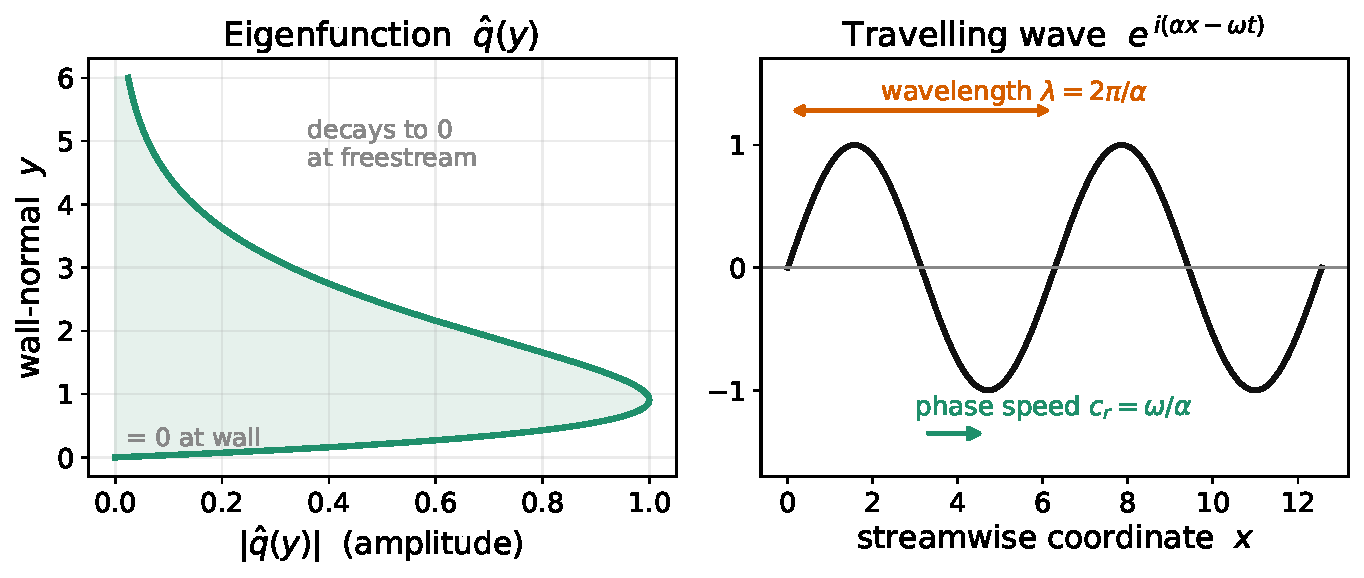
\includegraphics[width=0.92\linewidth]{fig_ansatz.pdf}
  \caption{The ansatz \eqref{eq:ansatz} factorises a disturbance $q'=\hatq(y)\,e^{\imag(\alpha x-\omega t)}$
  into a wall-normal \emph{shape} $\hatq(y)$ (left; zero at the wall, decaying at the edge --- the
  eigenfunction) times a travelling wave in $x$ (right; wavelength $2\pi/\alpha$, phase speed $c_r=\Real(c)$).}
\end{figure}

\section{The four disturbance equations}\label{sec:eqs}
\problembox{These are the linear ODEs in $y$ for $\hatu,\hatv,\hatT,\hatp$. Fixing one of $\alpha$ or
$\omega$ real makes the other (through $c$ or $\alpha$) the eigenvalue. Every overbarred quantity is a
known base-flow coefficient; all transport derivatives ($\mathrm d\mu/\mathrm dT$, $\mathrm d\kappa/\mathrm dT$,
\dots) are evaluated at the local mean temperature $\bar T(y)$ and are therefore known functions of $y$.}

The form assembled in \texttt{pymack/temporal\_solver.py} follows. Momentum and energy are divided by
$\bar\rho$; write the viscous prefactor $\nuR\equiv1/(\Ree\,\bar\rho)$. Throughout, every $\bar\rho$ is the
base-flow density, i.e.\ the diagonal field $\bar\rho(y)=1/\bar T(y)$ --- this single substitution applies
uniformly inside $\nuR$, $\mathcal C_\kappa$, and $\mathcal C_d$ below.

\paragraph{(C) Continuity $+$ equation of state.}
\begin{equation}\label{eq:cont}
  \imag\alpha\hatu+\D\hatv-\frac{\bar T'}{\bar T}\hatv
  +\imag\alpha(\bar U-c)\Big(\gamma\Mae^2\hatp-\frac{\hatT}{\bar T}\Big)=0 .
\end{equation}

\paragraph{(X) Streamwise momentum.}
\begin{equation}\label{eq:xmom}
\begin{aligned}
  \imag\alpha(\bar U-c)\hatu+\bar U'\hatv+\imag\alpha\bar\rho^{-1}\hatp
  =\nuR\Big[&\bar\mu\big(\D^2-\tfrac43\alpha^2\big)\hatu+\bar\mu'\D\hatu
     +\imag\alpha\big(\tfrac13\bar\mu\D+\bar\mu'\big)\hatv\\
   &+\tfrac{\mathrm d\mu}{\mathrm dT}\big(\bar U''+\bar U'\D\big)\hatT
     +\tfrac{\mathrm d^2\mu}{\mathrm dT^2}\bar U'\bar T'\hatT\Big] .
\end{aligned}
\end{equation}

\paragraph{(Y) Wall-normal momentum.}
\begin{equation}\label{eq:ymom}
\begin{aligned}
  \imag\alpha(\bar U-c)\hatv+\bar\rho^{-1}\D\hatp
  =\nuR\Big[&\bar\mu\big(\tfrac43\D^2-\alpha^2\big)\hatv+\tfrac43\bar\mu'\D\hatv
   +\imag\alpha\big(\tfrac13\bar\mu\D-\tfrac23\bar\mu'\big)\hatu
   +\imag\alpha\tfrac{\mathrm d\mu}{\mathrm dT}\bar U'\hatT\Big] .
\end{aligned}
\end{equation}

\paragraph{(E) Energy (temperature).}
\begin{equation}\label{eq:energy}
  \imag\alpha(\bar U-c)\hatT+\bar T'\hatv+(\gamma-1)\bar\rho^{-1}\big(\imag\alpha\hatu+\D\hatv\big)
  =\mathcal C_\kappa\mathcal L_c\hatT
   +\mathcal C_d\Big[2\bar\mu\bar U'\big(\D\hatu+\imag\alpha\hatv\big)
     +\tfrac{\mathrm d\mu}{\mathrm dT}\big(\bar U'\big)^2\hatT\Big],
\end{equation}
\begin{equation}
  \mathcal L_c=\D^2-\alpha^2
   +\tfrac1{\bar\kappa}\tfrac{\mathrm d\kappa}{\mathrm dT}\big(2\bar T'\D+\bar T''\big)
   +\tfrac1{\bar\kappa}\tfrac{\mathrm d^2\kappa}{\mathrm dT^2}\big(\bar T'\big)^2,\quad
  \mathcal C_\kappa=\frac{\gamma\bar\mu}{\mathit{Pr}\,\Ree\,\bar\rho},\quad
  \mathcal C_d=\frac{\gamma(\gamma-1)\Mae^2}{\Ree\,\bar\rho}.
\end{equation}

\paragraph{Reading the equations.}
\begin{itemize}[nosep,leftmargin=1.6em]
  \item $\imag\alpha(\bar U-c)$ is \emph{convection by the mean relative to the wave speed}; it vanishes at
        the \textbf{critical layer} $\bar U=c_r$, where the inviscid form of the equations becomes singular ---
        which is why that layer governs much of the instability physics.
  \item $\D,\D^2$ are wall-normal derivatives; $-\alpha^2$ comes from $\partial_x^2\!\mapsto\!-\alpha^2$.
  \item the $\nuR=1/(\Ree\bar\rho)$ terms are \emph{viscous} (the $\tfrac43,\tfrac13$ are Stokes's bulk
        viscosity; \S\ref{sec:spatial} generalises this to a ratio $\lambda/\mu=1.2$).
  \item the $\mathrm d\mu/\mathrm dT,\mathrm d\kappa/\mathrm dT$ terms are \emph{temperature-dependent transport} ---
        essential at hypersonic speeds.
  \item $\mathcal C_\kappa\mathcal L_c\hatT$ is heat conduction; $\mathcal C_d[\cdots]$ is viscous dissipation.
\end{itemize}

%=====================================================================
\part*{Part IV --- Turning equations into matrices}
\addcontentsline{toc}{section}{Part IV --- Turning equations into matrices}
%=====================================================================
\bridge{Part III left four coupled ODEs in $y$ with known base-flow coefficients but no closed-form
solution. Part IV converts them into a finite matrix a computer can handle.}

\section{Chebyshev collocation, from scratch}\label{sec:cheb}
\problembox{Replace the wall-normal derivative $\D$ by a finite matrix so the disturbance ODEs become
linear algebra; each continuous amplitude $\hatq(y)$ becomes a vector of its values at chosen grid points.}

\paragraph{Why Chebyshev?} For smooth functions a polynomial interpolant through Chebyshev points converges
\emph{exponentially}, so few points give many digits. The Chebyshev--Gauss--Lobatto (GLL) nodes on $[-1,1]$,
\begin{equation}\label{eq:gll}
  \xi_j=\cos\!\Big(\frac{\pi j}{N}\Big),\quad j=0,1,\dots,N,
\end{equation}
cluster near the ends $\xi=\pm1$. \textbf{Node ordering matters:} $\xi_0=+1$ and $\xi_N=-1$, so $j$ runs
from $+1$ down to $-1$.

\paragraph{The differentiation matrix.} One polynomial of degree $\le N$ passes through the values
$\{f(\xi_j)\}$; differentiating and evaluating at the nodes is linear, $f'(\xi_j)\approx\sum_kD_{jk}f(\xi_k)$,
with (Don \& Solomonoff; \texttt{spectral.py:chebyshev\_D})
\begin{equation}\label{eq:Dformula}
  D_{jk}=\frac{c_j}{c_k}\frac{(-1)^{j+k}}{\xi_j-\xi_k}\ (j\neq k),\qquad
  D_{jj}=-\!\!\sum_{k\neq j}D_{jk},\qquad c_0=c_N=2,\ c_{\text{else}}=1 .
\end{equation}
The diagonal is set so each row sums to zero (a constant function has zero slope); $c_0=c_N=2$ accounts for
the doubled weight of the two endpoints.
\plain{$D$ turns ``the list of function values'' into ``the list of slope values.'' It is dense --- every
node's slope uses every other node's value --- which is why the final stability matrices are dense.}

\paragraph{A 3-point worked example.} For $N=2$, $\xi=(1,0,-1)$ and \eqref{eq:Dformula} gives
\begin{equation}
  D=\begin{bmatrix}1.5&-2&0.5\\0.5&0&-0.5\\-0.5&2&-1.5\end{bmatrix},\qquad
  f'(\xi_1)\approx\tfrac12f(\xi_0)-\tfrac12f(\xi_2)\ \text{(centred difference).}
\end{equation}
The second derivative on $[-1,1]$ is the matrix square, $D^2_\xi=D_\xi D_\xi$ (\emph{not} the physical
$D_1$ squared --- see below).

\paragraph{Mapping to the physical layer.} The flow lives on $y\in[0,y_{\max}]$ with points clustered at the
\emph{wall}. The algebraic map (Malik 1990; \texttt{spectral.py:map\_domain}) is
\begin{equation}\label{eq:map}
  y(\xi)=L\,\frac{1+\xi}{1-\xi+2L/y_{\max}},\qquad L=\frac{y_{\max}}{6}\ (\text{stretching parameter}).
\end{equation}
This sends $\xi=+1$ (node $j{=}0$) to $y=y_{\max}$ (\textbf{freestream}) and $\xi=-1$ (node $j{=}N$) to
$y=0$ (\textbf{wall}); the grid median sits at $y(\xi{=}0)=y_{\max}/8$ and roughly half the points lie below
$y\approx L$. By the chain rule, with $\xi_y=1/y_\xi$ and $\xi_{yy}=-y_{\xi\xi}/y_\xi^3$, the physical
operators are
\begin{equation}\label{eq:Dmats}
  D_1=\operatorname{diag}(\xi_y)\,D_\xi,\qquad
  D_2=\operatorname{diag}(\xi_y^2)\,D_\xi^2+\operatorname{diag}(\xi_{yy})\,D_\xi .
\end{equation}
\remark{Common pitfall.}{The chain rule is applied to the \emph{computational} second-derivative matrix
$D_\xi^2=D_\xi D_\xi$, then mapped by \eqref{eq:Dmats}. The physical $D_2$ is \emph{not} $D_1D_1$.}

The physical domain must reach well past the boundary layer, so the truncation is set as a \emph{multiple of
the boundary-layer scale}, $y_{\max}=m\,(\delta^*/L^*)$, with $m\approx8$--$12$ for the wall-trapped second
mode and larger ($m\approx35$--$45$) for the more diffuse first mode; the bare values $y_{\max}=6$/$12$ are
only a fallback. The default resolution is $N=128$ ($n{=}N{+}1{=}129$); $N$ is a free accuracy parameter, and
because the method is spectral the eigenvalue converges \emph{exponentially} in $N$ (Figure~\ref{fig:conv}).

\begin{figure}[h]\centering
  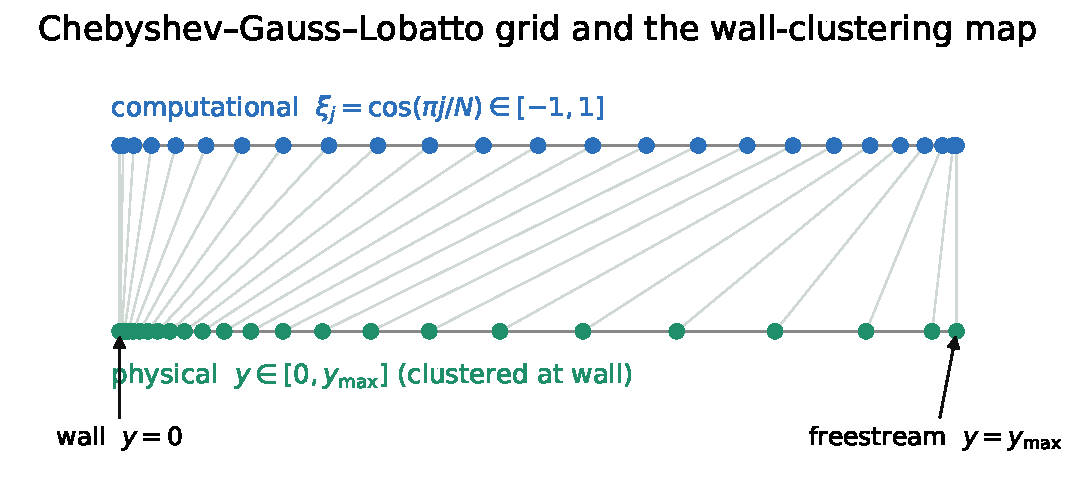
\includegraphics[width=0.92\linewidth]{fig_cheb_grid.pdf}
  \caption{The GLL nodes $\xi_j=\cos(\pi j/N)$ on $[-1,1]$ (top) map by Eq.~\eqref{eq:map} to the physical
  grid $y\in[0,y_{\max}]$ (bottom), piling up at the wall ($\xi=-1$) where eigenfunctions vary fastest.}
\end{figure}
\begin{figure}[h]\centering
  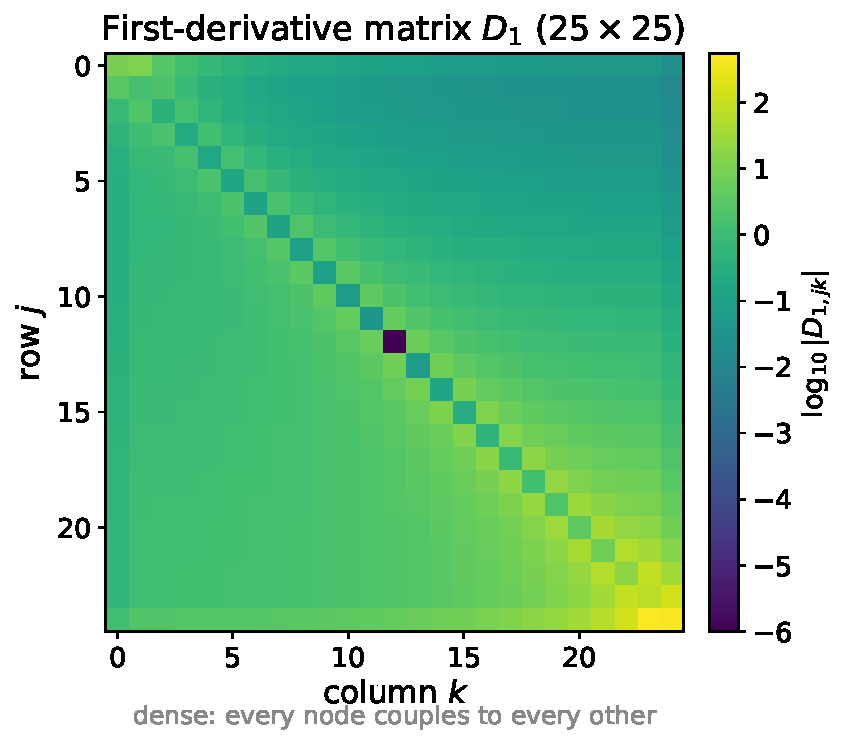
\includegraphics[width=0.45\linewidth]{fig_diffmat.pdf}\hfill
  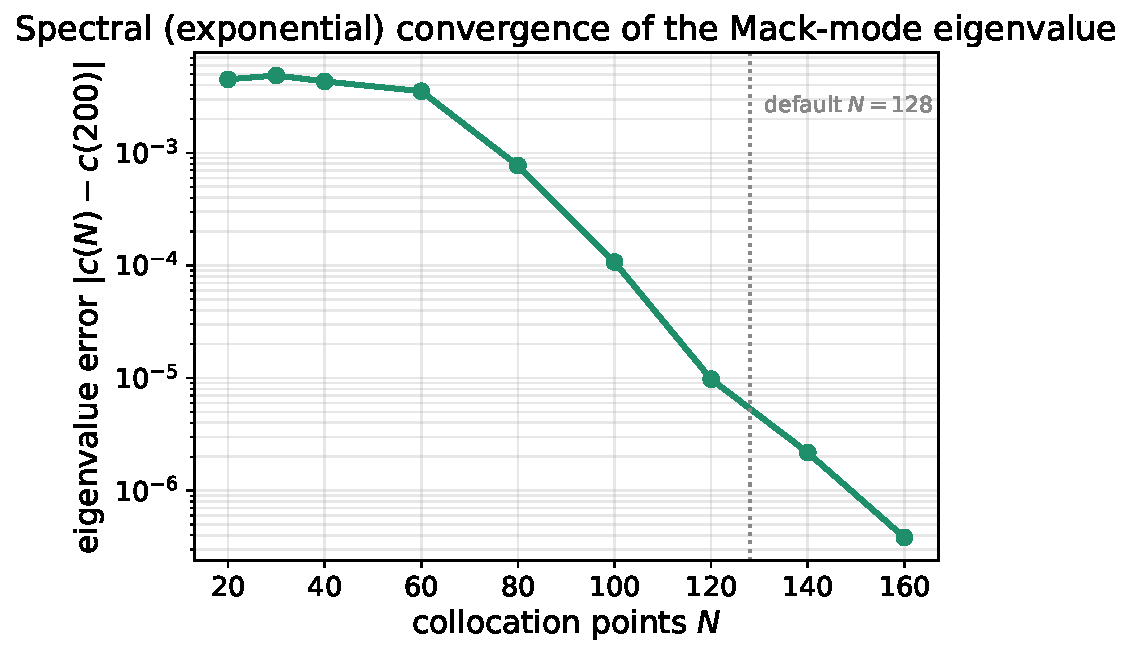
\includegraphics[width=0.49\linewidth]{fig_convergence.pdf}
  \caption{\emph{Left:} the physical first-derivative matrix $D_1$ ($25\times25$ here) is dense ($\log_{10}$
  of the entry magnitudes shown); spectral accuracy couples every node to every other. \emph{Right:} the
  payoff --- the worked-example eigenvalue error $|c(N)-c(200)|$ falls \emph{exponentially} with $N$ (a
  straight line on this semilog axis), so the default $N=128$ already gives many digits.}\label{fig:conv}
\end{figure}

\section{Assembling the operator and its boundary conditions}\label{sec:assemble}
\problembox{Stack the four nodal-value vectors into one length-$4n$ unknown and turn
Eqs.~\eqref{eq:cont}--\eqref{eq:energy} into one $4n\times4n$ matrix (two matrices, for the generalised
problem). Then overwrite the wall/freestream rows with boundary conditions.}

Each amplitude becomes a length-$n$ vector of nodal values; the four are stacked,
$\boldsymbol\phi=[\hatu;\hatv;\hatT;\hatp]\in\mathbb C^{4n}$. In every equation $\D\to D_1$, $\D^2\to D_2$,
and each mean coefficient becomes a diagonal matrix (e.g.\ $\bar U\to\operatorname{diag}(\bar U(y_j))$). Each
of the four equations contributes one block-row of four $n\times n$ blocks; the operator is the $4\times4$
array of blocks (Figure~\ref{fig:blocks}).

\paragraph{The eigenvalue split (which terms go where).} For the temporal problem (\S\ref{sec:temporal})
the only place $c$ appears is the factor $\imag\alpha(\bar U-c)$. Writing each such factor as
$\imag\alpha\bar U-c\,(\imag\alpha)$ splits the operator: the $\imag\alpha\bar U$ part stays in $A$, the
$c$-coefficient $-\imag\alpha$ goes into $B$. Equivalently $B=-\partial(\text{operator})/\partial c$. The
result is that \textbf{$A$ is the full block matrix whose rows are exactly Eqs.~\eqref{eq:cont}--\eqref{eq:energy}}
(coefficients moved to one side), and $B$ has only five non-zero blocks:
\begin{equation}\label{eq:Bblocks}
  B_{(C,\hatT)}=-\frac{\imag\alpha}{\bar T},\quad
  B_{(C,\hatp)}=\imag\alpha\gamma\Mae^2,\quad
  B_{(X,\hatu)}=\imag\alpha,\quad
  B_{(Y,\hatv)}=\imag\alpha,\quad
  B_{(E,\hatT)}=\imag\alpha .
\end{equation}
(The continuity row contributes \emph{two} $B$-blocks, on $\hatp$ and $\hatT$ --- the eigenvalue multiplies
the state-law pressure/temperature terms there, not a convective velocity.) Reading the $A$-blocks straight
off the four equations, a few representative ones are
\begin{equation}\label{eq:Ablocks}
  A_{(C,\hatu)}=\imag\alpha I,\quad
  A_{(C,\hatv)}=D_1-\tfrac{\bar T'}{\bar T},\quad
  A_{(X,\hatp)}=\imag\alpha\bar\rho^{-1},\quad
  A_{(Y,\hatp)}=\bar\rho^{-1}D_1,\quad
  A_{(E,\hatT)}=\imag\alpha\bar U-\mathcal C_\kappa\mathcal L_c-\mathcal C_d\tfrac{\mathrm d\mu}{\mathrm dT}(\bar U')^2 ,
\end{equation}
and every other block is the corresponding coefficient in Eqs.~\eqref{eq:cont}--\eqref{eq:energy} with
$\D\to D_1,\D^2\to D_2$. The pressure column of the energy row is zero ($A_{(E,\hatp)}=0$).

\begin{figure}[h]\centering
  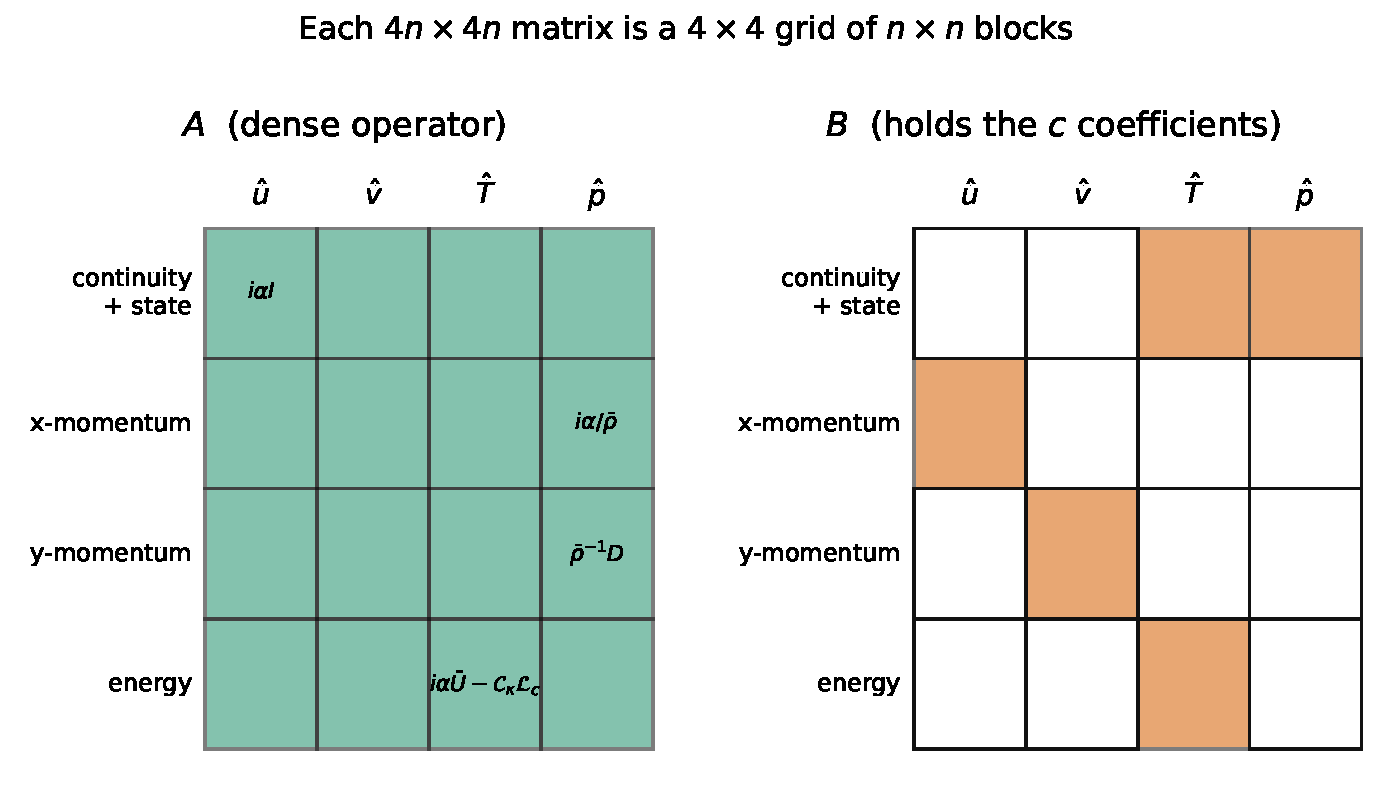
\includegraphics[width=0.95\linewidth]{fig_blocks.pdf}
  \caption{Block structure of $A\boldsymbol\phi=cB\boldsymbol\phi$. Rows = the four equations
  (continuity, $x$-mom, $y$-mom, energy); columns = the four fields $\hatu,\hatv,\hatT,\hatp$. \emph{Shaded
  = non-zero block.} $A$ (left) is block-dense; $B$ (right) holds only the five blocks of
  Eq.~\eqref{eq:Bblocks} --- every term carrying the eigenvalue $c$.}\label{fig:blocks}
\end{figure}

\paragraph{Boundary conditions = row replacement, with explicit indices.} A collocation row says ``the
equation holds at node $y_j$.'' At the wall and freestream we overwrite those rows. With the stacking
$\boldsymbol\phi=[\hatu;\hatv;\hatT;\hatp]$, field block $b\in\{0,1,2,3\}$ occupies global indices
$bn,\dots,bn+n-1$, and (from the ordering above) local index $0$ is the freestream, local index $n{-}1$ the
wall. Hence:
\begin{center}\small
\begin{tabular}{@{}llll@{}}
\toprule
condition & field & global row & row becomes \\
\midrule
no-slip (wall)        & $\hatu$ & $n-1$    & identity ($\hatu=0$)\\
no-slip (wall)        & $\hatv$ & $2n-1$   & identity ($\hatv=0$)\\
thermal (wall)        & $\hatT$ & $3n-1$   & identity ($\hatT=0$, isothermal) \emph{or} $D_1[\text{wall},:]$ ($\D\hatT=0$, adiabatic)\\
decay (freestream)    & $\hatu$ & $0$      & identity\\
decay (freestream)    & $\hatv$ & $n$      & identity\\
decay (freestream)    & $\hatT$ & $2n$     & identity\\
\bottomrule
\end{tabular}
\end{center}
The same rows of $B$ are zeroed so the constraint is algebraic; $\hatp$ carries no explicit boundary row.
\remark{Getting this backwards silently fails.}{Because $\xi_0=+1\to y_{\max}$ and $\xi_N=-1\to y=0$, node
index $0$ is the freestream and index $n{-}1$ is the wall --- the opposite of the naive guess. Swapping them
produces plausible-looking but wrong eigenvalues.}

\begin{figure}[h]\centering
  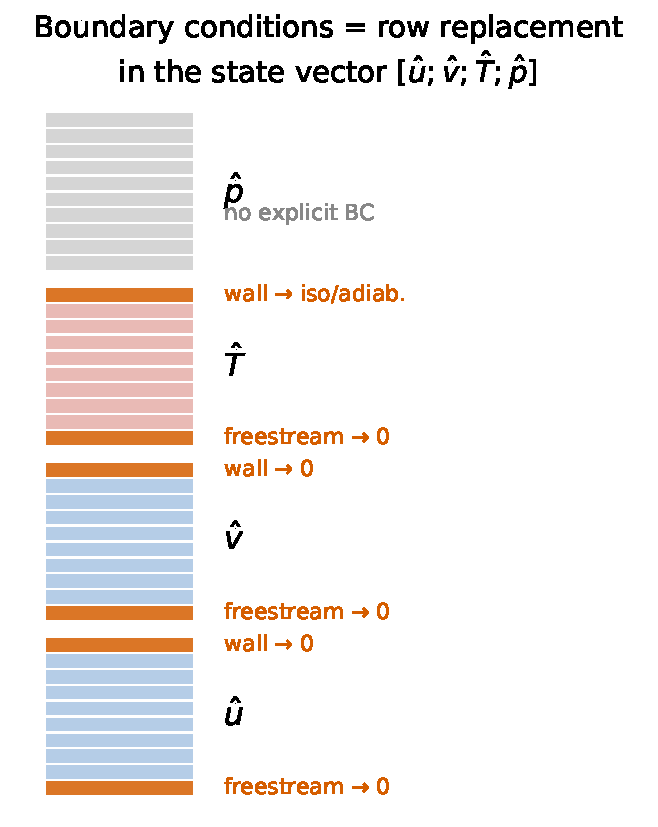
\includegraphics[width=0.32\linewidth]{fig_bc_rows.pdf}
  \caption{The boundary conditions as row replacement: the stacked state $[\hatu;\hatv;\hatT;\hatp]$ with the
  six overwritten rows highlighted (wall and freestream for $\hatu,\hatv,\hatT$); $\hatp$ carries no boundary
  row. Note index $0$ is the freestream and $n{-}1$ the wall.}
\end{figure}

%=====================================================================
\part*{Part V --- The eigenvalue problems}
\addcontentsline{toc}{section}{Part V --- The eigenvalue problems}
%=====================================================================
\bridge{The matrices are built, so ``does the wave grow?'' is now finite linear algebra. There are two
equivalent ways to pose it, depending on which of $\alpha,\omega$ we hold real.}

\section{Temporal problem: a generalised eigenvalue problem}\label{sec:temporal}
\problembox{\textbf{Given} a real wavenumber $\alpha$, \textbf{find} the complex phase speed $c$ and shape
$\boldsymbol\phi$. \textbf{Equation:} the four disturbance equations. \textbf{Eigenvalue:} $c$.
\textbf{Growth:} $\omega_i=\alpha\Imag(c)$.}

With $A,B$ from \S\ref{sec:assemble} this is a \textbf{generalised eigenvalue problem}
\begin{equation}\label{eq:tEVP}
  A\boldsymbol\phi=cB\boldsymbol\phi,\qquad A,B\in\mathbb C^{4n\times4n},
\end{equation}
solved directly by the QZ algorithm (\texttt{scipy.linalg.eig}), which returns all $4n$ eigenvalues at once.
\plain{An ordinary eigenproblem is $A\phi=c\phi$; a \emph{generalised} one allows a second matrix $B$ on the
right. The discrete eigenvector $\boldsymbol\phi$ is just the eigenfunction $\hatq(y)$ sampled at the grid
points --- ``eigenfunction'' and ``eigenvector'' are the continuous and discrete names for the same shape.}

A disturbance $\propto e^{\imag\alpha(x-ct)}$ with $\alpha$ real behaves as $e^{\alpha c_it}$ in time, so
\begin{equation}\label{eq:tgrowth}
  c_i=\Imag(c)>0\ \Rightarrow\ \textbf{unstable (grows in time)},\qquad c_r=\Real(c)=\text{wave speed.}
\end{equation}
The wave speed classifies the mode: a first (viscous/Tollmien--Schlichting) mode has $c_r\!\approx\!0.3$--$0.6$;
a second (Mack) mode has $c_r\!\approx\!1-1/\Mae$. The raw spectrum is filtered to
$\Real(c)\in(-0.5,1.5)$, $|\Imag(c)|<0.5$ and sorted by $c_i$.

\begin{figure}[h]\centering
  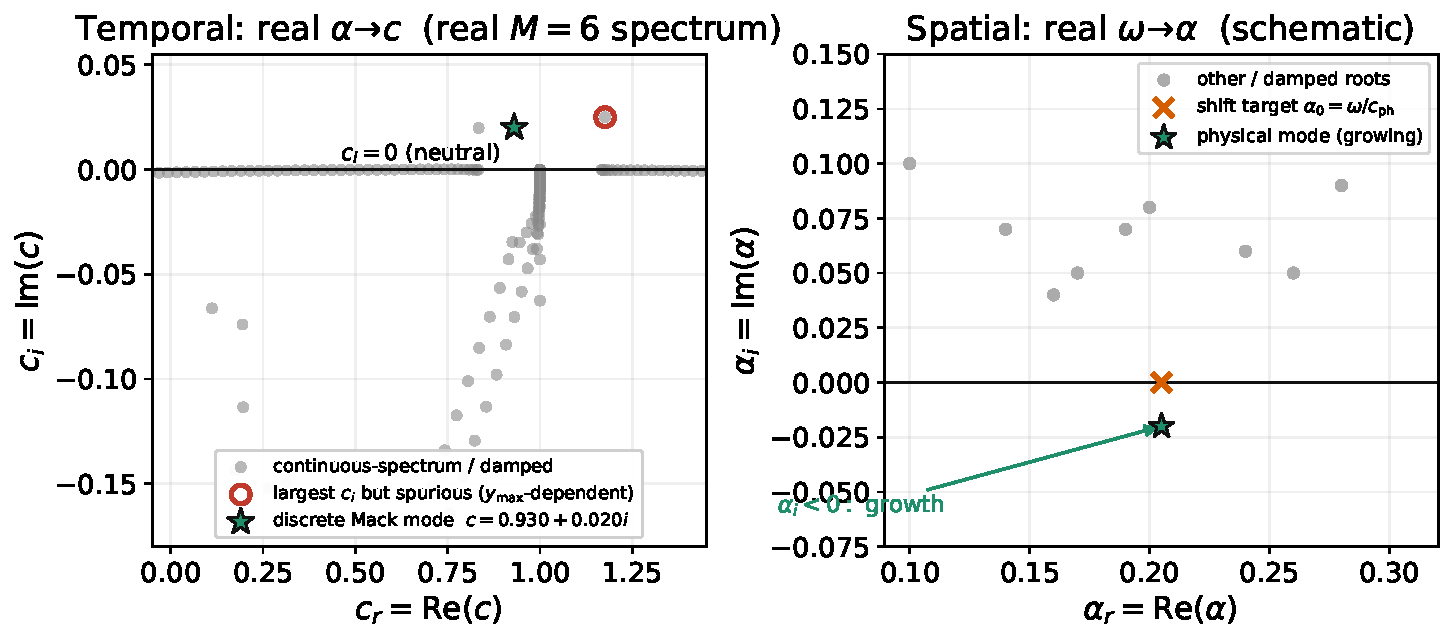
\includegraphics[width=0.95\linewidth]{fig_evp_planes.pdf}
  \caption{Where the eigenvalues live. \emph{Left (temporal):} input real $\alpha$; the phase speeds $c$
  populate the complex plane; the physical discrete mode sits above the line $c_i=\Imag(c)=0$ (unstable)
  while the continuous spectrum is damped. \emph{Right (spatial, explained in \S\ref{sec:spatial}):} input
  real $\omega$; the wavenumbers $\alpha$ are sought near a shift target $\alpha_0$; the physical mode has
  $\alpha_i<0$, i.e.\ growth.}\label{fig:planes}
\end{figure}

\section{Spatial problem: a quadratic eigenvalue problem}\label{sec:spatial}
\problembox{\textbf{Given} a real frequency $\omega$, \textbf{find} the complex wavenumber $\alpha$ and
shape. \textbf{Equation:} the same physics grouped by powers of $\alpha$. \textbf{Eigenvalue:} $\alpha$.
\textbf{Growth:} $\sigma=-\Imag(\alpha)$.}

A real source forces a fixed frequency and the disturbance grows in \emph{space}. Now $\omega$ is real and
$\alpha$ is the unknown; because viscous/conduction terms carry $\partial_x^2\!\mapsto\!-\alpha^2$, $\alpha$
appears \emph{quadratically}. Grouping the discretised Eqs.~\eqref{eq:cont}--\eqref{eq:energy} by powers of
$\alpha$ (substitute $\D\to D_1$, $\D^2\to D_2$, coefficients $\to$ diagonals, then collect $\alpha^0,\alpha^1,\alpha^2$)
gives a \textbf{quadratic eigenvalue problem} (QEP)
\begin{equation}\label{eq:qep}
  \big(C_0+\alpha C_1+\alpha^2C_2\big)\boldsymbol\phi=0 .
\end{equation}

\paragraph{Opening up $C_0,C_1,C_2$ (complete listing).} The spatial assembler (\texttt{equations.py}) uses
the \emph{enthalpy} energy form --- so $\hatp$ appears explicitly via $\D p'/\D t$ and the temperature
equation differs from \eqref{eq:energy} --- and a bulk-viscosity ratio $\lambda/\mu=1.2$. The resulting
viscous coefficients are
\begin{equation}
  c_{\alpha^2}=\tfrac{2(2+\lambda/\mu)}{3}=2.13,\qquad
  c_\times=\tfrac{1+2\lambda/\mu}{3}=1.13,\qquad
  c_a=\tfrac{2(\lambda/\mu-1)}{3}=0.13 \quad\text{(Mack Eq.~8.5)} .
\end{equation}
Because this closure is \emph{not} obtained by re-grouping \eqref{eq:cont}--\eqref{eq:energy}, here are
\emph{all} non-zero blocks, transcribed from \texttt{equations.py}. Write $\nuR=1/(\Ree\bar\rho)$ for the
viscous/conduction prefactor and $d_R=(\gamma-1)\Mae^2\nuR$ for the dissipation prefactor; each entry below
is the operator acting on the named field in that equation's block-row.
{\footnotesize
\begin{itemize}[leftmargin=2.6em,itemsep=2pt]
\item[\emph{(C)}] $C_0\!:\ \hatv\!\to D_1-\tfrac{\bar T'}{\bar T},\ \ \hatT\!\to\tfrac{\imag\omega}{\bar T},\ \ \hatp\!\to-\imag\omega\gamma\Mae^2$.\quad
  $C_1\!:\ \hatu\!\to\imag I,\ \ \hatT\!\to-\tfrac{\imag\bar U}{\bar T},\ \ \hatp\!\to\imag\gamma\Mae^2\bar U$.\quad $C_2\!:$ none.
\item[\emph{(X)}] $C_0\!:\ \hatu\!\to-\imag\omega-\nuR(\bar\mu D_2+\bar\mu'D_1),\ \ \hatv\!\to\bar U',\ \
  \hatT\!\to-\nuR\big[\tfrac{\mathrm d\mu}{\mathrm dT}(\bar U''+\bar U'D_1)+\tfrac{\mathrm d^2\mu}{\mathrm dT^2}\bar U'\bar T'\big]$.\quad
  $C_1\!:\ \hatu\!\to\imag\bar U,\ \ \hatv\!\to-\imag\nuR(c_\times\bar\mu D_1+\bar\mu'),\ \ \hatp\!\to\imag\bar\rho^{-1}$.\quad
  $C_2\!:\ \hatu\!\to c_{\alpha^2}\nuR\bar\mu$.
\item[\emph{(Y)}] $C_0\!:\ \hatv\!\to-\imag\omega-c_{\alpha^2}\nuR(\bar\mu D_2+\bar\mu'D_1),\ \ \hatp\!\to\bar\rho^{-1}D_1$.\quad
  $C_1\!:\ \hatu\!\to-\imag\nuR(c_\times\bar\mu D_1+c_a\bar\mu'),\ \ \hatv\!\to\imag\bar U,\ \ \hatT\!\to-\imag\nuR\tfrac{\mathrm d\mu}{\mathrm dT}\bar U'$.\quad
  $C_2\!:\ \hatv\!\to\nuR\bar\mu$.
\item[\emph{(E)}] $C_0\!:\ \hatu\!\to-2d_R\bar\mu\bar U'D_1,\ \ \hatv\!\to\bar T',\ \
  \hatT\!\to-\imag\omega-\nuR\big[\bar\kappa D_2+2\bar\kappa'D_1+\tfrac{\mathrm d\kappa}{\mathrm dT}\bar T''+\tfrac{\mathrm d^2\kappa}{\mathrm dT^2}(\bar T')^2\big]-d_R\tfrac{\mathrm d\mu}{\mathrm dT}(\bar U')^2,\ \ \hatp\!\to\imag\omega(\gamma-1)\Mae^2\bar\rho^{-1}$.\quad
  $C_1\!:\ \hatv\!\to-2\imag d_R\bar\mu\bar U',\ \ \hatT\!\to\imag\bar U,\ \ \hatp\!\to-\imag(\gamma-1)\Mae^2\bar U\bar\rho^{-1}$.\quad
  $C_2\!:\ \hatT\!\to\nuR\bar\kappa$.
\end{itemize}}
\noindent All other blocks are zero. The temporal closure \eqref{eq:cont}--\eqref{eq:energy} (Stokes
$\tfrac43,\tfrac13$ factors, temperature energy row) and this spatial closure (enthalpy row, $\lambda/\mu=1.2$)
differ only in the bulk-viscosity treatment and the energy-equation arrangement; both approximate the same
physical mode and agree on it to within discretisation error.

\paragraph{Companion linearisation.} A QEP becomes an ordinary (generalised) problem of \emph{twice} the
size by introducing $\boldsymbol\psi=\alpha\boldsymbol\phi$ (\texttt{solver.py}):
\begin{equation}\label{eq:companion}
  \underbrace{\begin{bmatrix}-C_1&-C_0\\ I&0\end{bmatrix}}_{\mathcal L}
  \begin{bmatrix}\boldsymbol\psi\\ \boldsymbol\phi\end{bmatrix}
  =\alpha\,\underbrace{\begin{bmatrix}C_2&0\\ 0&I\end{bmatrix}}_{\mathcal R}
  \begin{bmatrix}\boldsymbol\psi\\ \boldsymbol\phi\end{bmatrix}.
\end{equation}
The lower block row enforces $\boldsymbol\psi=\alpha\boldsymbol\phi$; the upper row then reproduces \eqref{eq:qep}.
The eigenvalue is $\alpha$ and the physical shape is the \emph{lower} half $\boldsymbol\phi$ (Figure~\ref{fig:companion}).
\remark{Why ``the lower half''.}{Since $\boldsymbol\psi=\alpha\boldsymbol\phi$ the two halves are parallel, so both
satisfy the QEP up to scaling; by convention $\boldsymbol\phi$ (lower half) is the one normalised as the eigenfunction.}

\begin{figure}[h]\centering
  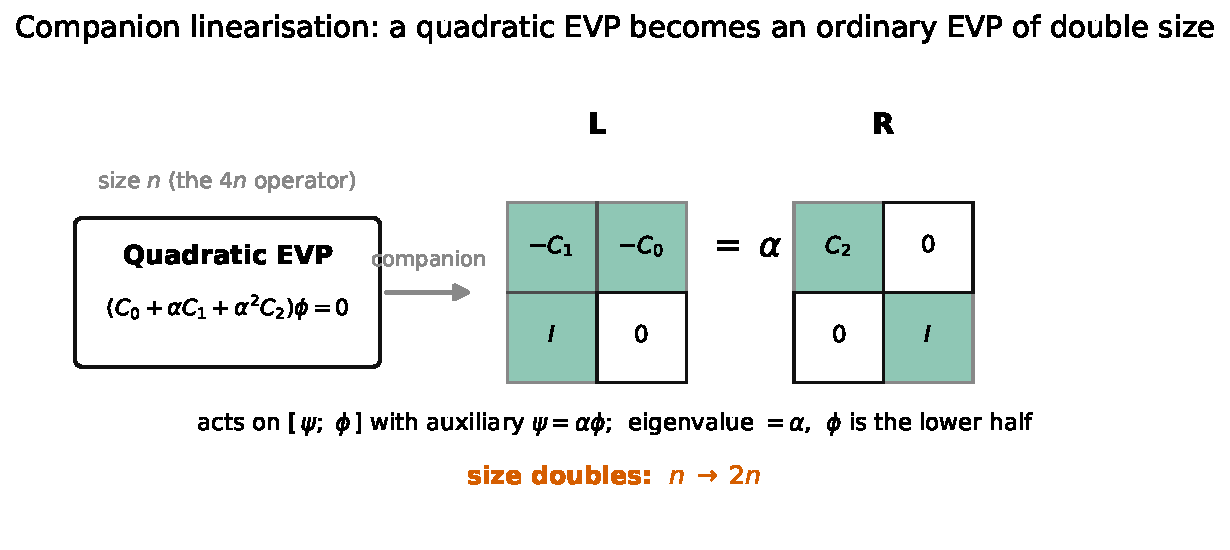
\includegraphics[width=0.9\linewidth]{fig_companion.pdf}
  \caption{Companion linearisation \eqref{eq:companion}: the $4n$-sized quadratic problem becomes an
  ordinary generalised problem of size $8n$ in $[\boldsymbol\psi;\boldsymbol\phi]$, with $\boldsymbol\psi=\alpha\boldsymbol\phi$.
  Its eigenvalue is exactly $\alpha$; the eigenfunction is the lower half.}\label{fig:companion}
\end{figure}

\paragraph{Shift--invert (which eigenvalue, cheaply).} We target the relevant branch with a shift
$\alpha_0=\omega/c_{\mathrm{ph}}$ ($c_{\mathrm{ph}}=1-1/\Mae$ for $\Mae>3$, else $\approx0.4$). Subtracting
$\alpha_0$ and inverting maps eigenvalues \emph{near} $\alpha_0$ to \emph{large} $\mu$, where
\begin{equation}\label{eq:shift}
  \text{eigenvalues of }(\mathcal L-\alpha_0\mathcal R)^{-1}\mathcal R\ \text{ are }\ \mu=\frac1{\alpha-\alpha_0},
  \qquad\Rightarrow\qquad \alpha=\alpha_0+\frac1\mu .
\end{equation}
So returning the largest-$|\mu|$ modes returns the wavenumbers nearest the physical one (one LU
factorisation; in \texttt{pyMack} a dense solve followed by selecting the $n_{\mathrm{modes}}{=}20$ nearest
$\alpha_0$, then sorting by $\Imag(\alpha)$). The amplitude $\propto e^{\imag\alpha x}=e^{\imag\alpha_rx}e^{-\alpha_ix}$, so
\begin{equation}\label{eq:sgrowth}
  \sigma=-\Imag(\alpha)=-\alpha_i>0\ \Rightarrow\ \textbf{unstable (grows downstream).}
\end{equation}

\remark{Alternative route --- Newton with a phase-speed seed.}{A more robust path when shift--invert
struggles (\texttt{solve\_spatial\_from\_temporal}): solve the \emph{temporal} problem at a real trial
$\alpha_r=\omega/c_{\mathrm{est}}$ ($c_{\mathrm{est}}=0.98$ for $\Mae>3$, else $0.35$), keeping only modes
that agree across two resolutions (tolerance $8\times10^{-3}$); form the seed
$\Imag(\alpha)\approx-\alpha_rc_i/c_r$ (a \emph{phase-speed} estimate --- the rigorous Gaster relation uses
the group velocity $c_g=\mathrm d\omega_r/\mathrm d\alpha_r$, but here it only seeds Newton, so precision is
unneeded); then Newton-iterate the dispersion residual $F(\alpha)=\alpha c(\alpha)-\omega=0$,
$\alpha^{(k+1)}=\alpha^{(k)}-F/F'$, with $F'=c+\alpha\,\mathrm dc/\mathrm d\alpha$ approximated by a finite
difference (step $10^{-5}$, tol $10^{-6}$, $\le20$ iterations). Both routes return the same
$\sigma=-\Imag(\alpha)$.}

\section{Which eigenvalue is physical?}\label{sec:modes}
\problembox{Given the full $4n$-element spectrum, identify the one eigenvalue that is a genuine
boundary-layer mode rather than continuous-spectrum noise.}

Besides the discrete boundary-layer modes the operator has a dense \textbf{continuous spectrum} --- on an
infinite domain these freestream disturbances form an unbroken band rather than isolated points, and the
finite grid renders them as a dense cluster. Two tests (\texttt{discrete\_mode.py}) keep only the physical
mode (Figure~\ref{fig:critlayer}):
\begin{enumerate}[nosep,leftmargin=1.8em]
  \item \textbf{Freestream decay}: a true boundary-layer eigenfunction decays as $y\to y_{\max}$, a
        continuous-spectrum one does not. Reject candidates whose edge-to-peak amplitude ratio exceeds
        $\sim\!0.06$.
  \item \textbf{Domain stationarity}: a genuine eigenvalue barely moves if the truncation changes. Recompute
        at two domain heights and keep modes whose $c$ matches to $\sim\!4\times10^{-3}$; accept growth rates
        with $|c_i|\lesssim0.05$ and $c_r$ in the physical band.
\end{enumerate}
\plain{These two tests are the difference between a clean growth rate and noise --- they are what let us
trust a single number out of the full $4n$-element spectrum (724 modes in the worked example of
\S\ref{sec:worked}, where the largest-growth eigenvalue is in fact spurious).}

\begin{figure}[h]\centering
  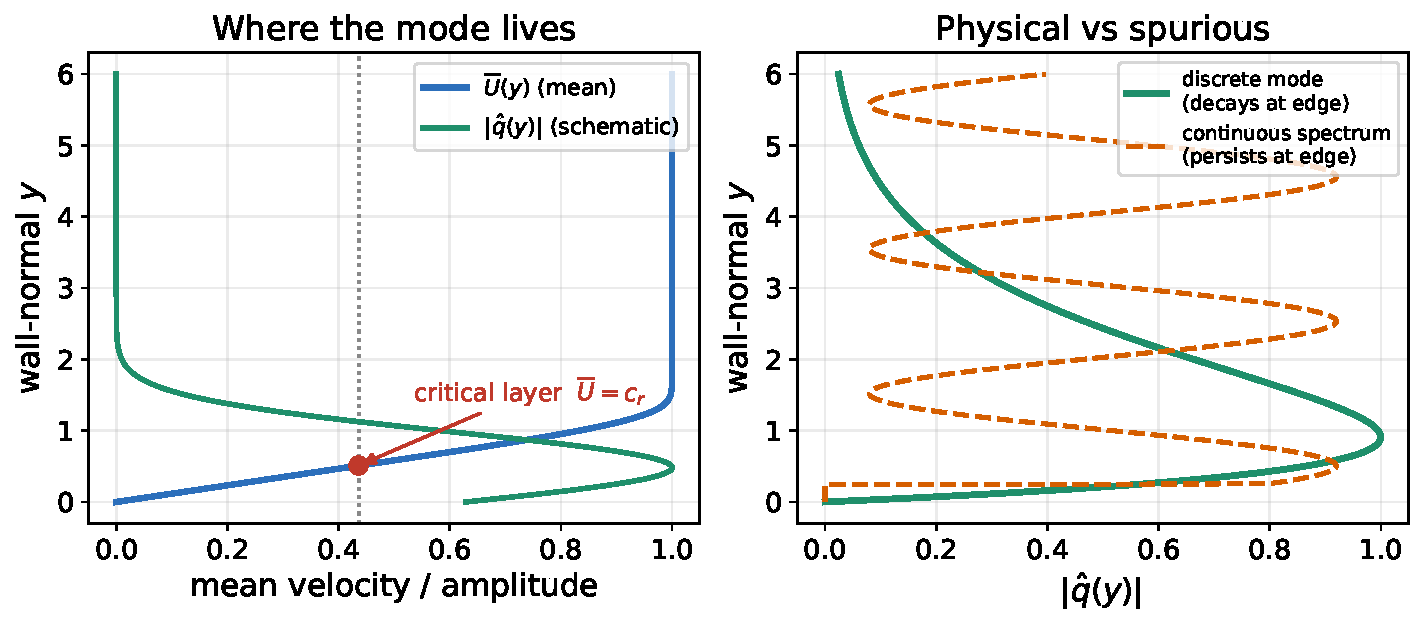
\includegraphics[width=0.95\linewidth]{fig_critlayer.pdf}
  \caption{\emph{Left:} the critical layer is where $\bar U(y)=c_r$; the mode's amplitude $|\hatq(y)|$ tends
  to peak near it. \emph{Right:} a discrete boundary-layer mode (solid) decays toward the freestream, while
  a continuous-spectrum mode (dashed) keeps oscillating to the edge --- the basis for the two acceptance
  tests.}\label{fig:critlayer}
\end{figure}

\section{Worked example: one temporal solve, start to finish}\label{sec:worked}
Take a strong Mack-mode case: $\Mae=6.0$, $R=5500$, $\alpha_L=0.174$, adiabatic wall, $L^*$ scaling,
$N=180$ ($n=181$, so the matrices are $4n=724$ wide). The wall-normal domain is
$y_{\max}=10\,(\delta^*/L^*)\approx128$ (\S\ref{sec:cheb}: the domain is a multiple of the boundary-layer
scale, not a bare number). Solving \eqref{eq:tEVP} returns 724 eigenvalues; after the physical filter the
six least-stable are
\begin{center}\small
\begin{tabular}{@{}rrrll@{}}
\toprule
$c_r$ & $c_i$ & $\omega_i=\alpha c_i$ & $y_{\max}$-stationary? & verdict \\
\midrule
$+1.176$ & $+0.0249$ & $+0.00434$ & no ($|\Delta c|\!\sim\!10^{-2}$) & spurious / continuous spectrum \\
$\mathbf{+0.930}$ & $\mathbf{+0.0200}$ & $\mathbf{+0.00348}$ & \textbf{yes} ($|\Delta c|\!\sim\!10^{-7}$) & \textbf{discrete Mack mode --- the answer} \\
$+0.834$ & $+0.0197$ & $+0.00343$ & no & continuous spectrum \\
$+0.740$ & $+0.0000$ & $\phantom{+}0.00000$ & --- & neutral continuous-spectrum cluster \\
$+0.720$ & $+0.0000$ & $\phantom{+}0.00000$ & --- & continuous spectrum \\
$+0.760$ & $+0.0000$ & $\phantom{+}0.00000$ & yes & stable discrete mode \\
\bottomrule
\end{tabular}
\end{center}
This is the trap the mode tests of \S\ref{sec:modes} exist to avoid: the \emph{largest}-growth eigenvalue
(row~1, $c_r=1.18$) is \emph{not} the answer --- it is spurious, its $c$ shifting by $\sim\!10^{-2}$ when the
domain height changes (and $c_r>1$ is unphysically supersonic). The physical answer is row~2, the
\textbf{Mack (second) mode} $c=0.930+0.0200\imag$: domain-stationary to $10^{-7}$, with an eigenfunction that
decays at the freestream (Figure~\ref{fig:eigfn}). Its growth rate is $\omega_i=\alpha c_i=+0.00348$
(unstable) and its phase speed $c_r=0.93$ is the second-mode value explained in \S\ref{sec:mechanisms}.

\begin{figure}[h]\centering
  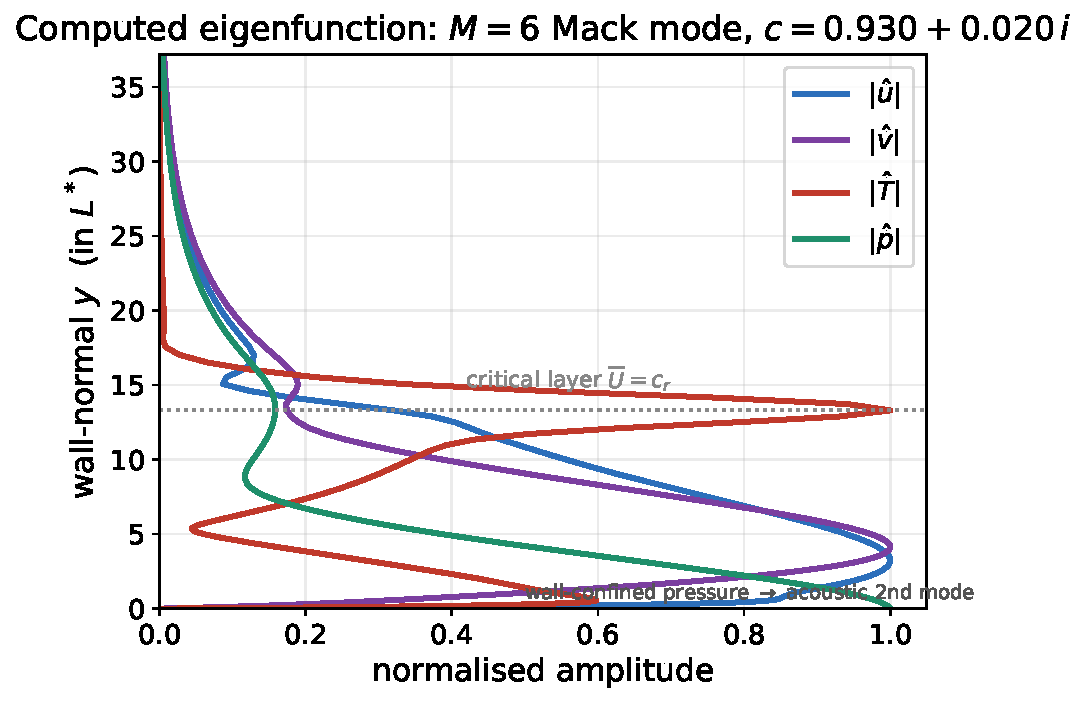
\includegraphics[width=0.58\linewidth]{fig_eigenfunctions.pdf}
  \caption{Computed eigenfunction of the worked-example Mack mode: the four amplitude fields
  $|\hatu|,|\hatv|,|\hatT|,|\hatp|$ vs $y$ (each normalised). $|\hatT|$ spikes at the critical layer
  ($\bar U=c_r$); $|\hatp|$ is wall-confined --- the acoustic signature of the second mode
  (\S\ref{sec:mechanisms}). All fields decay at the freestream, confirming a discrete mode.}\label{fig:eigfn}
\end{figure}

\emph{This single $\omega_i>0$ is one point ``inside'' the neutral curve: repeating the solve across an
$(R,\alpha)$ grid and finding where $\omega_i$ crosses zero traces the neutral curve of Part VI.} (All
numbers reproduce from \texttt{solve\_temporal\_2d}.)

\section{What the modes \emph{are}: two instability mechanisms}\label{sec:mechanisms}
We have a growth rate; now the \emph{physics} behind the mode labels, so that $c=0.930+0.0200\imag$ becomes an
understood wave, not a number.

\paragraph{First (Tollmien--Schlichting) mode.} At \emph{low} speed the first mode is a viscous instability
($c_r\!\approx\!0.3$--$0.6$): counter-intuitively, viscosity introduces a phase lag between $u'$ and $v'$ near
the wall, so the Reynolds stress $-\bar\rho\,\overline{u'v'}$ no longer averages to zero and draws energy from
the mean shear. As the Mach number rises, compressibility creates a generalised inflection point (below) and
the first mode becomes increasingly \emph{inviscid/inflectional} --- governed by that point, with viscosity
then often \emph{stabilising}. It is the dominant instability only up to $\Mae\!\approx\!4$.

\paragraph{Second (Mack) mode --- a trapped acoustic wave.} Above $\Mae\!\approx\!4$ a second, usually
stronger, instability appears: it is essentially \emph{a sound wave trapped between the wall and the
``relative sonic line''}, reflecting in a near-wall acoustic cavity (Figure~\ref{fig:trap}). This one picture
explains three facts we earlier had to accept blindly:
\begin{itemize}[nosep,leftmargin=1.6em]
  \item its phase speed is $c_r\!\approx\!1-1/\Mae$ --- the \emph{limiting} ``edge-sonic'' value at which the
        wave is sonic relative to the edge flow, which is why the shift target $\alpha_0=\omega/(1-1/\Mae)$ of
        \S\ref{sec:spatial} works; the realised $c_r$ sits somewhat above this and varies along the branch
        ($0.93$ vs $1-1/6=0.83$ here), so it is a guide, not an exact value;
  \item it is \emph{frequency-tuned}: like any resonator its wavelength is set by the cavity thickness, so the
        most-amplified wavelength is $\sim\!2\delta$, giving the order-of-magnitude scaling
        $f\!\sim\!U_e/2\delta$ --- the second-mode frequency rises as the layer thins downstream;
  \item its eigenfunction (Figure~\ref{fig:eigfn}) has a \emph{wall-peaked pressure} --- the acoustic field in
        the cavity.
\end{itemize}

\paragraph{The organising quantity: relative Mach number.} Both pictures live in the \textbf{relative Mach
number} $M_{\rm rel}(y)=(\bar U-c_r)/\bar a(y)$, with $\bar a=\sqrt{\bar T}/\Mae$ the local sound speed. The
critical layer is $M_{\rm rel}=0$; the relative sonic line is $|M_{\rm rel}|=1$; the second-mode acoustic
cavity is the near-wall region where $|M_{\rm rel}|>1$ (Figure~\ref{fig:trap}).

\paragraph{Why a compressible layer is unstable at all (the generalised inflection point).} Rayleigh's
theorem: an inviscid \emph{incompressible} shear flow needs a velocity inflection point ($\bar U''=0$) to be
unstable. Compressibility generalises this (Lees--Lin) to the \textbf{generalised inflection point} where
$\tfrac{d}{dy}(\bar\rho\,\bar U')=0$ --- the necessary condition for the inviscid \emph{first} mode.
Aerodynamic heating puts a hot, low-density layer near the wall (the $\bar T$ bulge in
Figure~\ref{fig:baseflow}, where the point is marked) and pushes that generalised inflection point up into the
layer --- giving the robust inviscid first-mode instability that low-speed layers lack. The \emph{second}
(Mack) mode needs no inflection point: its existence condition is instead the near-wall relative-supersonic
cavity ($|M_{\rm rel}|>1$) above.

\paragraph{The wall-cooling reversal (the key design lever).} Cooling the wall \emph{stabilises} the first
mode (it weakens the near-wall viscous mechanism) but \emph{destabilises} the second (it thickens the
relative-supersonic cavity and raises the tuned frequency). This is why cold-walled hypersonic vehicles are
second-mode dominated --- and why the solver carries an isothermal-wall option.

\paragraph{Phase vs group velocity.} $c_r$ is the \emph{phase} speed (crest speed); energy travels at the
\emph{group} velocity $c_g=\mathrm d\omega_r/\mathrm d\alpha_r$. It is $c_g$ that rigorously links temporal to
spatial growth, which is why the phase-speed Gaster estimate of \S\ref{sec:spatial} is only a seed.

\begin{figure}[h]\centering
  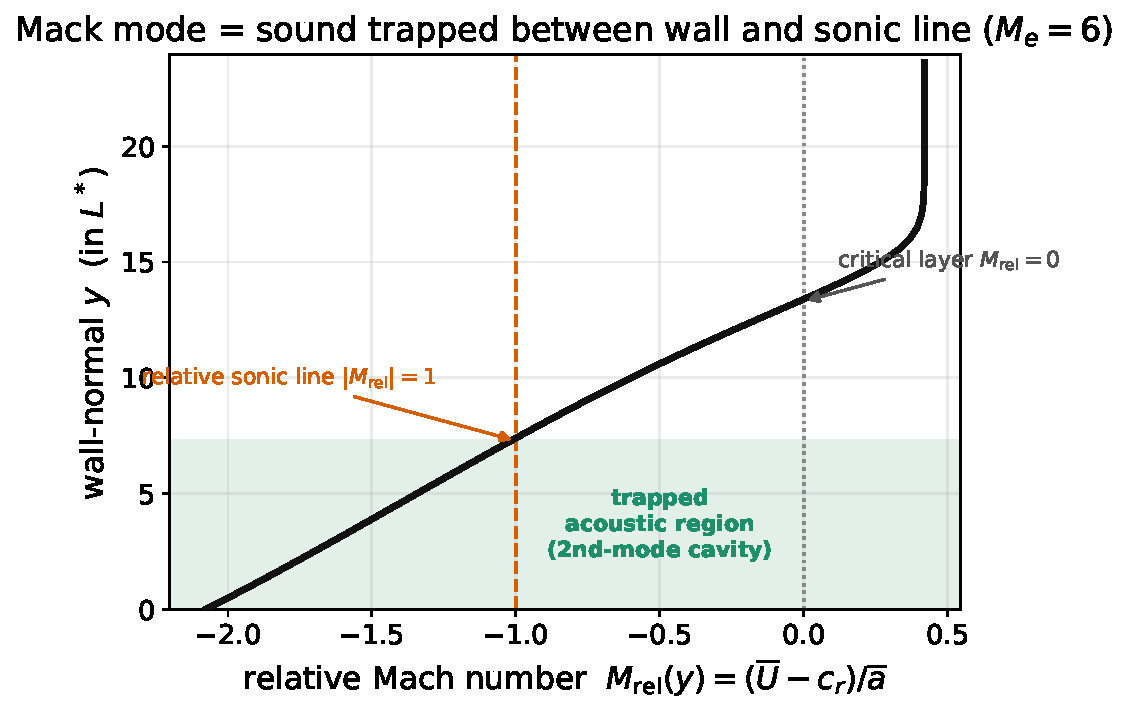
\includegraphics[width=0.6\linewidth]{fig_acoustic_trapping.pdf}
  \caption{The second-mode mechanism, for the worked-example mode. The relative Mach number
  $M_{\rm rel}(y)=(\bar U-c_r)/\bar a$ is supersonic ($|M_{\rm rel}|>1$, shaded) in a near-wall cavity bounded
  by the wall and the relative sonic line ($|M_{\rm rel}|=1$), and passes through zero at the critical layer.
  The Mack mode is a sound wave trapped in that cavity.}\label{fig:trap}
\end{figure}

\noindent A compact comparison places any computed eigenvalue at a glance:
\begin{center}\small
\renewcommand{\arraystretch}{1.2}
\begin{tabular}{@{}>{\raggedright\arraybackslash}p{3.1cm}>{\raggedright\arraybackslash}p{5.1cm}>{\raggedright\arraybackslash}p{5.1cm}@{}}
\toprule
 & \textbf{First (TS) mode} & \textbf{Second (Mack) mode} \\
\midrule
mechanism & viscous (low speed) $\to$ inviscid inflectional (high speed) & trapped acoustic wave (wall--sonic line) \\
phase speed $c_r$ & $0.3$--$0.6$ & $\approx 1-1/\Mae$ (here $0.93$) \\
dominant when & low speed, $\Mae\lesssim4$ & high speed, $\Mae\gtrsim4$ \\
frequency & broadband & tuned, $f\sim U_e/2\delta$ \\
existence criterion & generalised inflection point (Lees--Lin) & relative-supersonic cavity, $|M_{\rm rel}|>1$ \\
wall cooling & stabilises & destabilises \\
most-unstable wave & oblique (3D) & 2D ($\psi=0$) \\
\bottomrule
\end{tabular}
\end{center}

%=====================================================================
\part*{Part VI --- Products: neutral curves and $N$-factors}
\addcontentsline{toc}{section}{Part VI --- Products}
%=====================================================================
\bridge{One solve gives one growth rate. Sweeping the solve over parameters produces the two engineering
outputs: the neutral curve (boundary of instability) and the $N$-factor (a transition predictor).}

\section{Neutral curves}\label{sec:neutral}
\problembox{Map the boundary between growth and decay: the locus where the growth rate is exactly zero.}

The neutral curve is $c_i(R,\alpha)=0$ (temporal) or $\sigma(R,\omega)=0$ (spatial); inside it the flow is
unstable. \texttt{pyMack} draws it in three steps:
\begin{enumerate}[nosep,leftmargin=1.8em]
  \item \textbf{Sweep} an $(R,\alpha)$ grid at fixed $\Mae$; at each node solve \eqref{eq:tEVP}, apply the
        mode tests (\S\ref{sec:modes}), store $c_i$ (\texttt{build\_*\_grid.py}). This is the field in
        Figure~\ref{fig:neutral}.
  \item \textbf{Extract} the zero contour with marching squares (a standard method for tracing a
        $c_i=0$ level set through a grid of values; \texttt{extract\_contours.py}); unresolved nodes are
        tagged stable so the loop closes.
  \item \textbf{Continuation} for hard branches: at low Mach the first-mode eigenvalue sinks into the
        continuous spectrum. \texttt{trace\_continuation.py} tracks it \emph{by proximity} --- from a clean
        seed it marches in $R$, follows the nearest $c$, and secant-solves $c_i=0$ at each step
        (continuation = using each converged eigenvalue as the guess for the next nearby parameter value).
\end{enumerate}

\begin{figure}[h]\centering
  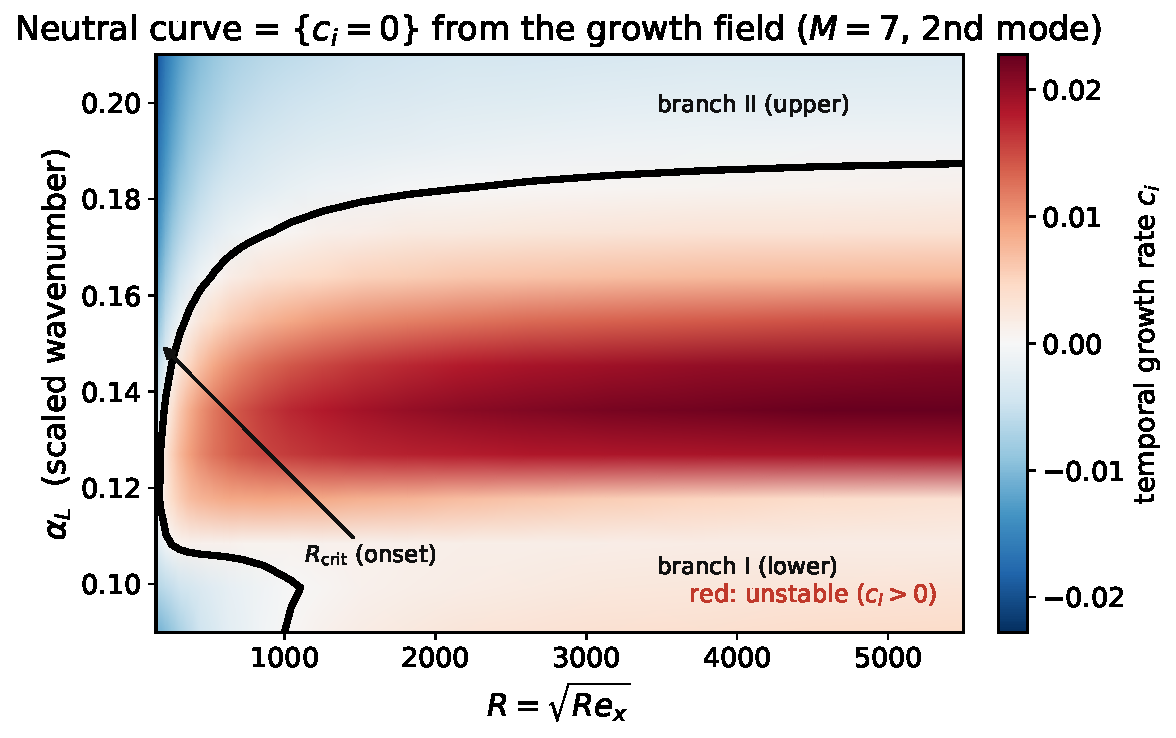
\includegraphics[width=0.7\linewidth]{fig_neutral_field.pdf}
  \caption{A real growth field $c_i(R,\alpha)$ from a parameter sweep ($\Mae=7$, second mode). Colour is the
  temporal growth $c_i$ (red $=$ unstable, $c_i>0$); the thick black curve is the neutral contour $c_i=0$
  that pyMack reports. Axes are the Mack variables $R=\sqrt{Re_x}$ and $\alpha_L=\alpha L^*$.}\label{fig:neutral}
\end{figure}

\section{$N$-factor and transition}\label{sec:nfactor}
\problembox{Convert local spatial growth into a single number predicting transition.}

What matters for transition is the \emph{accumulated} amplification of a fixed-frequency disturbance. For a
chosen $F$, solve the spatial problem (\S\ref{sec:spatial}) at successive stations to get
$\sigma_L=-\Imag(\alpha_L)$ --- this is the same spatial growth $\sigma$ of Eq.~\eqref{eq:sgrowth}, expressed
in the $L^*$ (Mack-length) scaling of Eq.~\eqref{eq:RF} --- and integrate from the lower neutral point $R_0$
(where $\sigma_L$ first turns positive):
\begin{equation}\label{eq:N}
  N(R)=\int_{R_0}^R\max(\sigma_L,0)\,\mathrm dR'\quad\text{(trapezoidal)},\qquad \frac{A(R)}{A(R_0)}=e^{N(R)} .
\end{equation}
The amplitude grows by $e^N$; transition is empirically expected near $N\approx9$--$11$ (the $e^N$ method;
\texttt{analysis.py}). For a cone, surface arc length is mapped to an equivalent $R$ before integrating.
\remark{$e^N$ is a correlation, not a criterion.}{The transition $N$ is \emph{not} universal: it depends on
the disturbance environment (flight $\sim$9--11; noisy conventional tunnels can transition at $N\!\sim\!4$--$6$).
It presumes a single dominant linear mode and stops at the onset of nonlinear breakdown, and it silently
absorbs the unknown initial amplitude set by receptivity (\S\ref{sec:scope}).}

\begin{figure}[h]\centering
  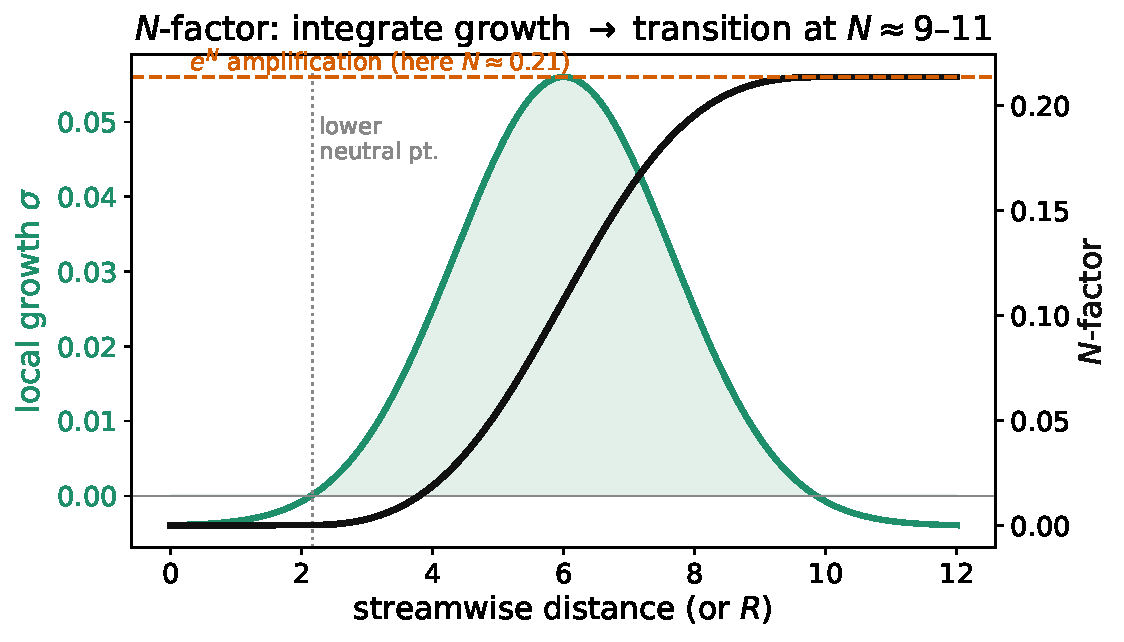
\includegraphics[width=0.66\linewidth]{fig_nfactor.pdf}
  \caption{The $N$-factor. \emph{Shaded/green (left axis):} local spatial growth $\sigma=-\alpha_i$, non-zero
  only between the two neutral points. \emph{Black (right axis):} its running integral $N(R)$, the exponent
  of the amplification $e^N$. Transition correlates with $N\approx9$--$11$.}
\end{figure}

\section{Scope and limitations}\label{sec:scope}
This document solves the \emph{2D, parallel-flow, modal} eigenvalue problem and converts its growth into an
$e^N$ estimate. That is one stage of transition (Figure~\ref{fig:roadmap}); a careful reader should keep four
idealizations in view:
\begin{enumerate}[nosep,leftmargin=1.9em]
  \item \textbf{Parallel flow.} Setting $\bar v=0$ and $y$-only coefficients neglects the $O(1/R)$ streamwise
        growth of the layer; the standard remedy is the \emph{Parabolised Stability Equations} (PSE), which
        march the disturbance downstream retaining slow $x$-variation.
  \item \textbf{Two-dimensionality.} The solver takes $\beta=0$. The most-unstable \emph{first} mode is
        oblique ($\psi\!\sim\!55^\circ$, Squire's theorem fails under compressibility), so 2D first-mode
        growth is a \emph{lower bound}; the \emph{second}/Mack mode is most unstable at $\psi=0$, so the 2D
        result is its physical maximum.
  \item \textbf{Modal analysis only.} Eigenvalues describe asymptotic growth; the non-normal operator also
        permits \emph{transient (algebraic) growth} that modal analysis misses, relevant to bypass and
        blunt-body paths.
  \item \textbf{Receptivity and $e^N$.} LST gives the amplification \emph{ratio} $A(R)/A(R_0)=e^N$, not the
        initial amplitude $A(R_0)$; setting that is the separate \emph{receptivity} problem, and $e^N$ is an
        environment-dependent correlation rather than a first-principles criterion.
\end{enumerate}
None of these affect the equations or numerics above; they bound their interpretation. The worked-example
second mode (\S\ref{sec:worked}) is captured faithfully by the 2D modal solver.

\section{Summary and replication checklist}\label{sec:summary}
\begin{center}\small
\renewcommand{\arraystretch}{1.25}
\begin{tabular}{@{}>{\raggedright\arraybackslash}p{2.7cm}>{\raggedright\arraybackslash}p{4.6cm}
>{\raggedright\arraybackslash}p{4.4cm}>{\raggedright\arraybackslash}p{2.4cm}@{}}
\toprule
\textbf{Goal} & \textbf{Problem solved} & \textbf{Method} & \textbf{Growth} \\
\midrule
Temporal growth, neutral curves
  & generalised EVP $A\boldsymbol\phi=cB\boldsymbol\phi$, real $\alpha$ (Eq.~\ref{eq:tEVP})
  & Chebyshev collocation $+$ QZ & $\alpha c_i$ \\
Spatial growth, $N$-factor
  & quadratic EVP $(C_0+\alpha C_1+\alpha^2C_2)\boldsymbol\phi=0$, real $\omega$ (Eq.~\ref{eq:qep})
  & companion $+$ shift--invert; or temporal $+$ Newton seed & $-\alpha_i$ \\
Neutral curve
  & $\{c_i=0\}$ over an $(R,\alpha)$ sweep
  & grid sweep $\to$ marching squares; continuation & --- \\
Transition
  & $N=\int\max(\sigma_L,0)\,\mathrm dR$ (Eq.~\ref{eq:N})
  & fixed-$F$ spatial march $+$ integration & --- \\
\bottomrule
\end{tabular}
\end{center}

\paragraph{To re-implement the solver from scratch.}
\begin{enumerate}[nosep,leftmargin=1.9em]
  \item Solve the base-flow boundary-value problem \eqref{eq:bl-mom}--\eqref{eq:blbc}; tabulate $\bar U,\bar T$ and derivatives.
  \item Build $\xi_j$ \eqref{eq:gll}, $D_\xi$ \eqref{eq:Dformula}, map to $y$ \eqref{eq:map}, form $D_1,D_2$ \eqref{eq:Dmats}.
  \item Assemble the $4\times4$ block operator from Eqs.~\eqref{eq:cont}--\eqref{eq:energy} (temporal: $A,B$ with the split \eqref{eq:Bblocks}; spatial: $C_0,C_1,C_2$).
  \item Overwrite the wall/freestream rows with the boundary conditions (\S\ref{sec:assemble} table), respecting the node ordering.
  \item Solve the eigenvalue problem (temporal \eqref{eq:tEVP} or spatial \eqref{eq:companion}); filter for the discrete mode (\S\ref{sec:modes}); read $c_i$ or $-\alpha_i$.
  \item Sweep parameters; extract $\{c_i=0\}$ for neutral curves, or integrate $-\alpha_i$ for $N$-factors.
\end{enumerate}

\bigskip
\noindent\emph{Code map.} base flow: \texttt{pymack/baseflow.py}; scales: \texttt{pymack/scales.py};
spectral operators: \texttt{pymack/spectral.py}; temporal assembly: \texttt{pymack/temporal\_solver.py};
spatial assembly: \texttt{pymack/equations.py}; solvers / companion / Newton: \texttt{pymack/solver.py};
mode selection: \texttt{discrete\_mode.py}; neutral-curve drivers and continuation:
\texttt{verification/.../build\_*\_grid.py}, \texttt{extract\_contours.py}, \texttt{trace\_continuation.py}.

\end{document}
